\documentclass[10pt,aspectratio=169]{beamer}

\usepackage[UTF8]{ctex}
\usepackage{amsmath,amssymb,booktabs,tabularx,array}
\usepackage{graphicx}
\usepackage{tikz}
\usepackage{xcolor}
\usepackage{hyperref}
\usepackage{xurl}

\usetheme{Madrid}
\usefonttheme{professionalfonts}
\setbeameroption{hide notes}
\setbeamertemplate{navigation symbols}{}
\setbeamertemplate{itemize items}[circle]

\definecolor{primary}{HTML}{0B5E75}
\definecolor{secondary}{HTML}{0173B2}
\definecolor{accent}{HTML}{D97706}
\definecolor{good}{HTML}{027A5B}
\definecolor{ink}{HTML}{17324D}
\definecolor{muted}{HTML}{667085}
\definecolor{pale}{HTML}{EAF3F8}
\definecolor{warm}{HTML}{FCF0DF}
\definecolor{grid}{HTML}{D0D5DD}

\setbeamercolor{structure}{fg=primary}
\setbeamercolor{title}{fg=white}
\setbeamercolor{subtitle}{fg=white!85}
\setbeamercolor{frametitle}{fg=white,bg=primary}
\setbeamercolor{block title}{fg=white,bg=primary}
\setbeamercolor{block body}{fg=ink,bg=pale}
\setbeamercolor{alerted text}{fg=accent}
\setbeamercolor{normal text}{fg=ink,bg=white}
\setbeamercolor{footline}{fg=white,bg=ink}

\setbeamertemplate{footline}{
  \leavevmode%
  \hbox{%
    \begin{beamercolorbox}[wd=.78\paperwidth,ht=2.7ex,dp=1.1ex,leftskip=1em]{footline}
      Stage 2 估计器比较
    \end{beamercolorbox}%
    \begin{beamercolorbox}[wd=.22\paperwidth,ht=2.7ex,dp=1.1ex,rightskip=1em plus1fil]{footline}
      \insertframenumber
    \end{beamercolorbox}%
  }
}

\graphicspath{{figures/}}
\newcommand{\method}[1]{\textsf{#1}}
\newcommand{\best}[1]{\textcolor{secondary}{\textbf{#1}}}
\newcommand{\keypoint}[1]{\textcolor{good}{\textbf{#1}}}
\newcommand{\caution}[1]{\textcolor{accent}{\textbf{#1}}}
\newcommand{\sourcefoot}[1]{\vspace{1mm}\par{\scriptsize\color{muted}来源：#1}}
\newcommand{\metriccard}[3]{%
  \begin{beamercolorbox}[rounded=true,sep=0.7em,wd=\linewidth]{block body}
    {\scriptsize\color{muted}#1}\par
    {\Large\bfseries\color{#3}#2}
  \end{beamercolorbox}}

\title{Stage 2：估计器如何选？}
\subtitle{从 168 个真实 Pythia 候选到可执行的后续实验配置}
\author{Parameter Importance Project}
\institute{Shanghai Jiao Tong University}
\date{2026 年 8 月 28 日}

\begin{document}

\begin{frame}[plain]
  \begin{tikzpicture}[remember picture,overlay]
    \fill[primary] (current page.south west) rectangle (current page.north east);
    \fill[secondary,opacity=.22] ([xshift=8.0cm]current page.south west)
      -- (current page.south east) -- (current page.north east)
      -- ([xshift=12.2cm]current page.north west) -- cycle;
    \fill[accent] ([yshift=0.72cm]current page.south west)
      rectangle ([yshift=0.86cm]current page.south east);
  \end{tikzpicture}
  \vspace{0.85cm}
  {\color{white}\Huge\bfseries Stage 2：估计器如何选？\par}
  \vspace{0.35cm}
  {\color{white!85}\Large 从 168 个真实 Pythia 候选到可执行的后续实验配置\par}
  \vspace{1.05cm}
  \begin{columns}[T,onlytextwidth]
    \column{0.57\textwidth}
      {\color{white}\large
        2 个模型 $\times$ 3 个阶段\\[2mm]
        4 个样本预算 $\times$ 7 种估计器}
    \column{0.38\textwidth}
      \begin{beamercolorbox}[rounded=true,sep=0.8em]{block body}
        \centering
        \textbf{默认答案}\\[1mm]
        {\Large\best{U-32, $B=32$}}
      \end{beamercolorbox}
  \end{columns}
  \vfill
  {\color{white!70}\small Parameter Importance Project \hfill 2026-08-28}
  \note{开场先给答案：如果今天只能带走一个配置，就是 U-32、B=32。接下来解释为什么这不是“每个 cell 都最好”，而是跨模型、跨阶段最稳健的统一选择。}
\end{frame}

\begin{frame}{结论先行：统一默认 + 阶段化例外}
  \begin{columns}[T,onlytextwidth]
    \column{0.32\textwidth}
      \metriccard{统一默认}{U-32}{secondary}
      \vspace{2mm}
      \metriccard{样本预算}{$B=32$}{good}
    \column{0.64\textwidth}
      \begin{block}{后续实验的最小决策规则}
        \begin{itemize}
          \item \best{初始化：U-8}，同时保留 Raw；
          \item \best{训练早期：U-32}；Pythia-14M 可特化为 Double、$B=64$；
          \item \best{中后期：U-16 或 U-32}，同时保留 Raw；
          \item Double 与 U-2 等价，只保留一个输出。
        \end{itemize}
      \end{block}
      \vspace{1mm}
      {\small 这是一套\keypoint{依据当前数据内容可执行}的估计器选择策略。}
  \end{columns}
  \sourcefoot{Stage 2 direct real-Pythia run，run id: pythia-grid-20260826T145530Z}
  \note{强调“统一默认”和“逐 cell 最优”是两个问题。U-32 的价值在稳健性；阶段化配置用来争取局部最低误差。后续所有图都围绕这两个层次展开。}
\end{frame}

\begin{frame}{我们比较了什么？}
  \begin{columns}[T,onlytextwidth]
    \column{0.56\textwidth}
      \resizebox{\linewidth}{!}{%
      \begin{tikzpicture}[x=1.05cm,y=.82cm,font=\small]
        \node[anchor=west,font=\bfseries\color{primary}] at (0,4.15) {完整实验矩阵};
        \foreach \x/\lab in {0/14M,1/31M} {
          \node[draw=grid,fill=pale,minimum width=.9cm,minimum height=.55cm] at (\x,3.35) {\lab};
        }
        \node[anchor=west] at (2.25,3.35) {$\times$};
        \foreach \y/\lab in {0/初始,1/早期,2/中后期} {
          \node[draw=grid,fill=white,minimum width=1.15cm,minimum height=.55cm] at (3.05+\y*1.15,3.35) {\lab};
        }
        \node[anchor=west] at (6.65,3.35) {$\times$};
        \foreach \y/\lab in {0/32,1/64,2/128,3/256} {
          \node[draw=grid,fill=warm,minimum width=.72cm,minimum height=.55cm] at (.1+\y*.83,2.25) {\lab};
        }
        \node[anchor=west] at (3.55,2.25) {$\times$};
        \node[draw=grid,fill=pale,minimum width=3.75cm,minimum height=.55cm] at (5.85,2.25)
          {Raw / Double / U-2 / 4 / 8 / 16 / 32};
        \node[anchor=west,font=\Large\bfseries\color{secondary}] at (0,1.05)
          {$2\times3\times4\times7=168$};
        \node[anchor=west,text=muted] at (0,.42) {个候选汇总};
      \end{tikzpicture}}
    \column{0.40\textwidth}
      \begin{block}{比较指标}
        \begin{itemize}
          \item MSE：主排序指标
          \item MAE：绝对误差
          \item Pearson：形状保持
          \item signed bias：系统偏差
          \item between-repetition variance：重复稳定性
          \item 壁钟时间 / 峰值显存
        \end{itemize}
      \end{block}
  \end{columns}
  \sourcefoot{除 31M 中后期、$B=64$ 的交付汇总为 $n=18$ 外，其余均为 $n=64$。}
  \note{这是范围页。候选数 168 指交付汇总的笛卡尔积，不是说 168 次训练。每个候选又聚合多次 repetition。需要明确唯一覆盖例外：31M 中后期 B=64 只交付续跑段 18 次。}
\end{frame}

\begin{frame}{估计器与读图口径}
  \begin{columns}[T,onlytextwidth]
    \column{0.55\textwidth}
      \begin{block}{三类估计器}
        \[
          \widehat I_{\mathrm{Raw}}
          =\left(\frac{1}{B}\sum_{i=1}^{B} g_i\right)^2
        \]
        \[
          \widehat I_{\mathrm{Double}}=\bar g_A\bar g_B
        \]
        \[
          \widehat I_{U,M}
          =\frac{\left(\sum_{m=1}^{M}\bar g_m\right)^2
          -\sum_{m=1}^{M}\bar g_m^2}{M(M-1)}
        \]
      \end{block}
    \column{0.41\textwidth}
      \begin{block}{如何判断“更好”}
        \begin{itemize}
          \item MSE / MAE：\best{越低越好}
          \item Pearson：\best{越接近 1 越好}
          \item 排名：在同一 cell、同一 $B$ 内比较
          \item 成本：profiler 同时算全部方法，\caution{不能拆分单方法耗时}
        \end{itemize}
      \end{block}
      \vspace{2mm}
      {\small\caution{关键不变量：}当 $M=2$ 时，U-2 与 Double 代数等价。}
  \end{columns}
  \note{公式只服务于解释。Raw 是先平均再平方；Double 用独立半样本乘积；U-M 用 M 组交叉项。后面 Double 和 U-2 曲线重合不是巧合，而是定义决定的实现不变量。}
\end{frame}

\begin{frame}{数据覆盖完整，但有一个交付边界}
  \centering
  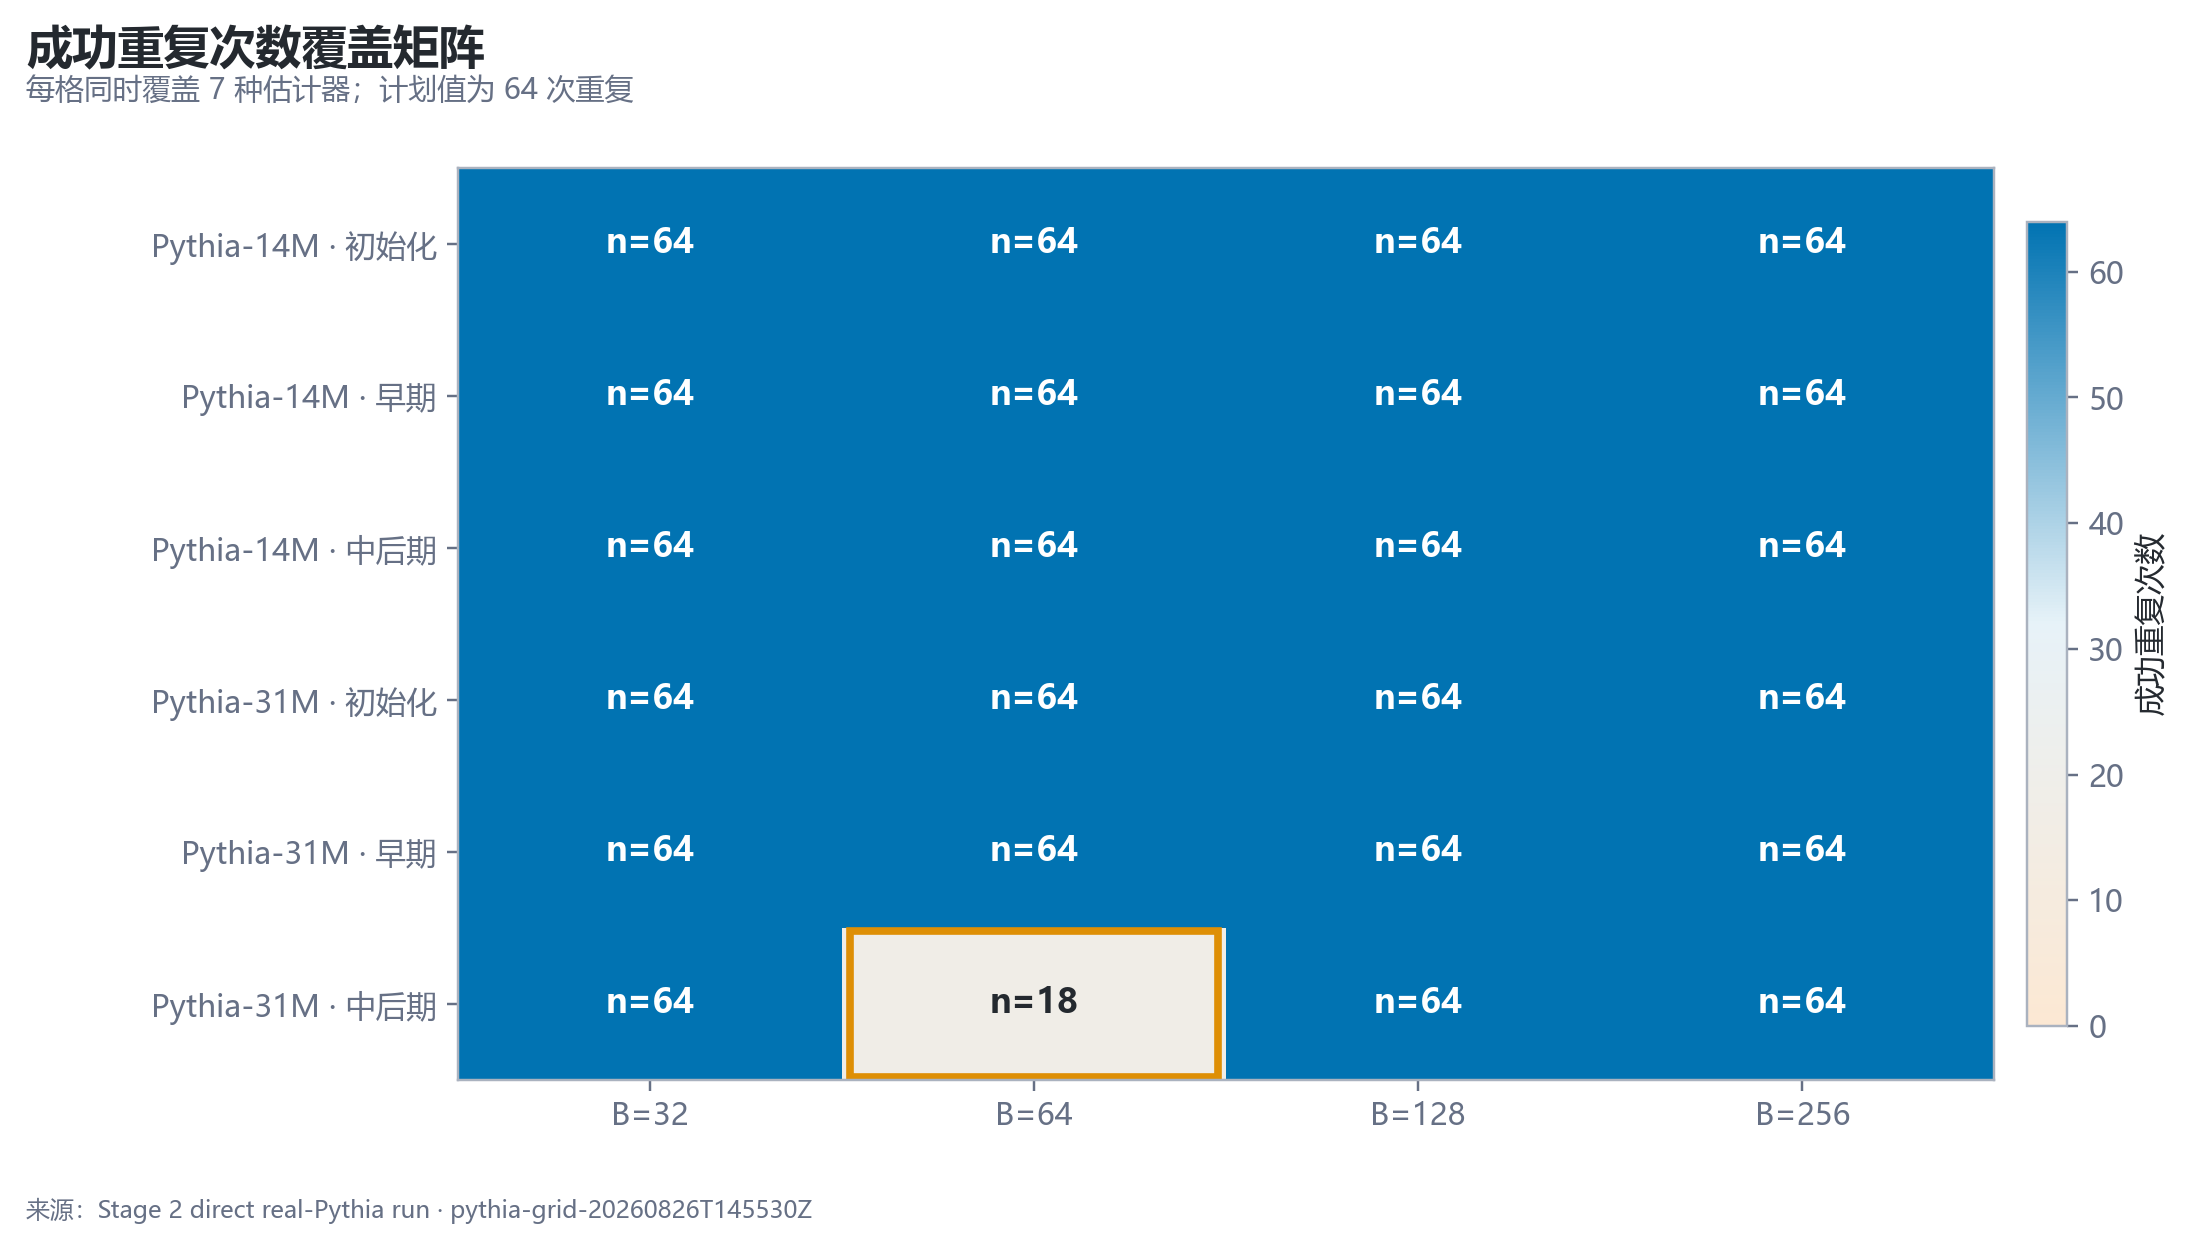
\includegraphics[height=.50\textheight,keepaspectratio]{fig01-coverage-matrix.png}
  \vspace{-1mm}
  \begin{beamercolorbox}[rounded=true,sep=.55em,wd=.88\textwidth]{block body}
    \centering
    23 个 cell--batch 汇总为 $n=64$；\quad
    \caution{31M 中后期、$B=64$ 为 $n=18$}
  \end{beamercolorbox}
  \sourcefoot{图中每格同时支持 7 种估计器；覆盖共 168 个候选。}
  \note{先确认数据是否足以“产生内容结论”：是。六个 cell、四个 B、七种方法均有汇总。唯一边界是一个 cell-batch 的 n 较小，因此不能把它和其他格子的置信程度视为完全相同。}
\end{frame}

\begin{frame}{六个 cell，出现五种最低 MSE 配置}
  \centering
  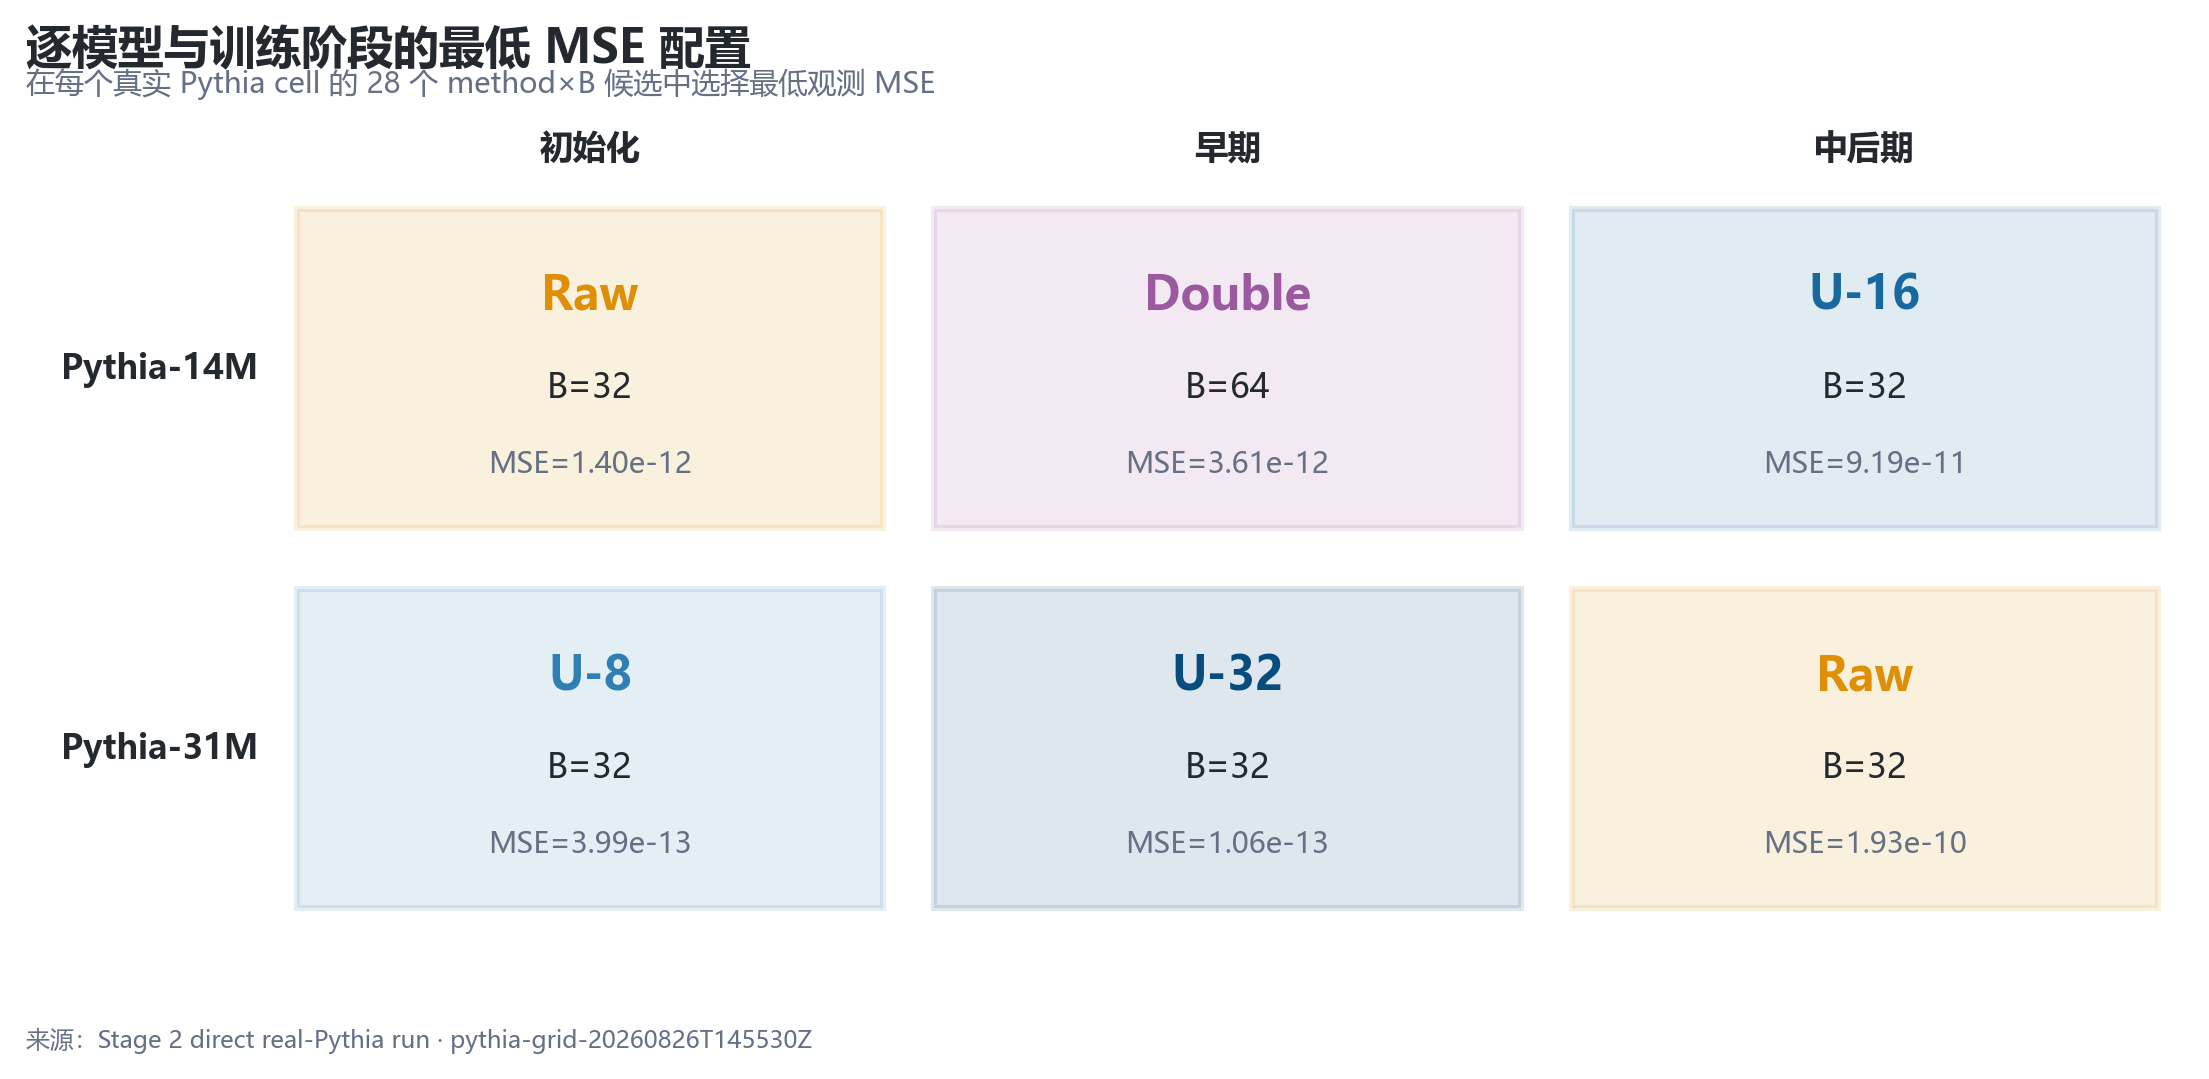
\includegraphics[width=.86\textwidth]{fig02-cell-winners.png}
  \begin{columns}[T,onlytextwidth]
    \column{.48\textwidth}
      {\small\best{14M：}Raw $\rightarrow$ Double $\rightarrow$ U-16}
    \column{.48\textwidth}
      {\small\best{31M：}U-8 $\rightarrow$ U-32 $\rightarrow$ Raw}
  \end{columns}
  \sourcefoot{每格为该模型与阶段的全局最低观测 MSE。}
  \note{这是最重要的“异质性”证据。没有方法在六个 cell 中包办冠军。模型规模和训练阶段都会改变最优配置，因此报告给的是“统一默认加阶段例外”，而不是声称存在普适最优。}
\end{frame}

\begin{frame}{跨场景稳定性：U-32 平均排名最好}
  \begin{columns}[T,onlytextwidth]
    \column{0.65\textwidth}
      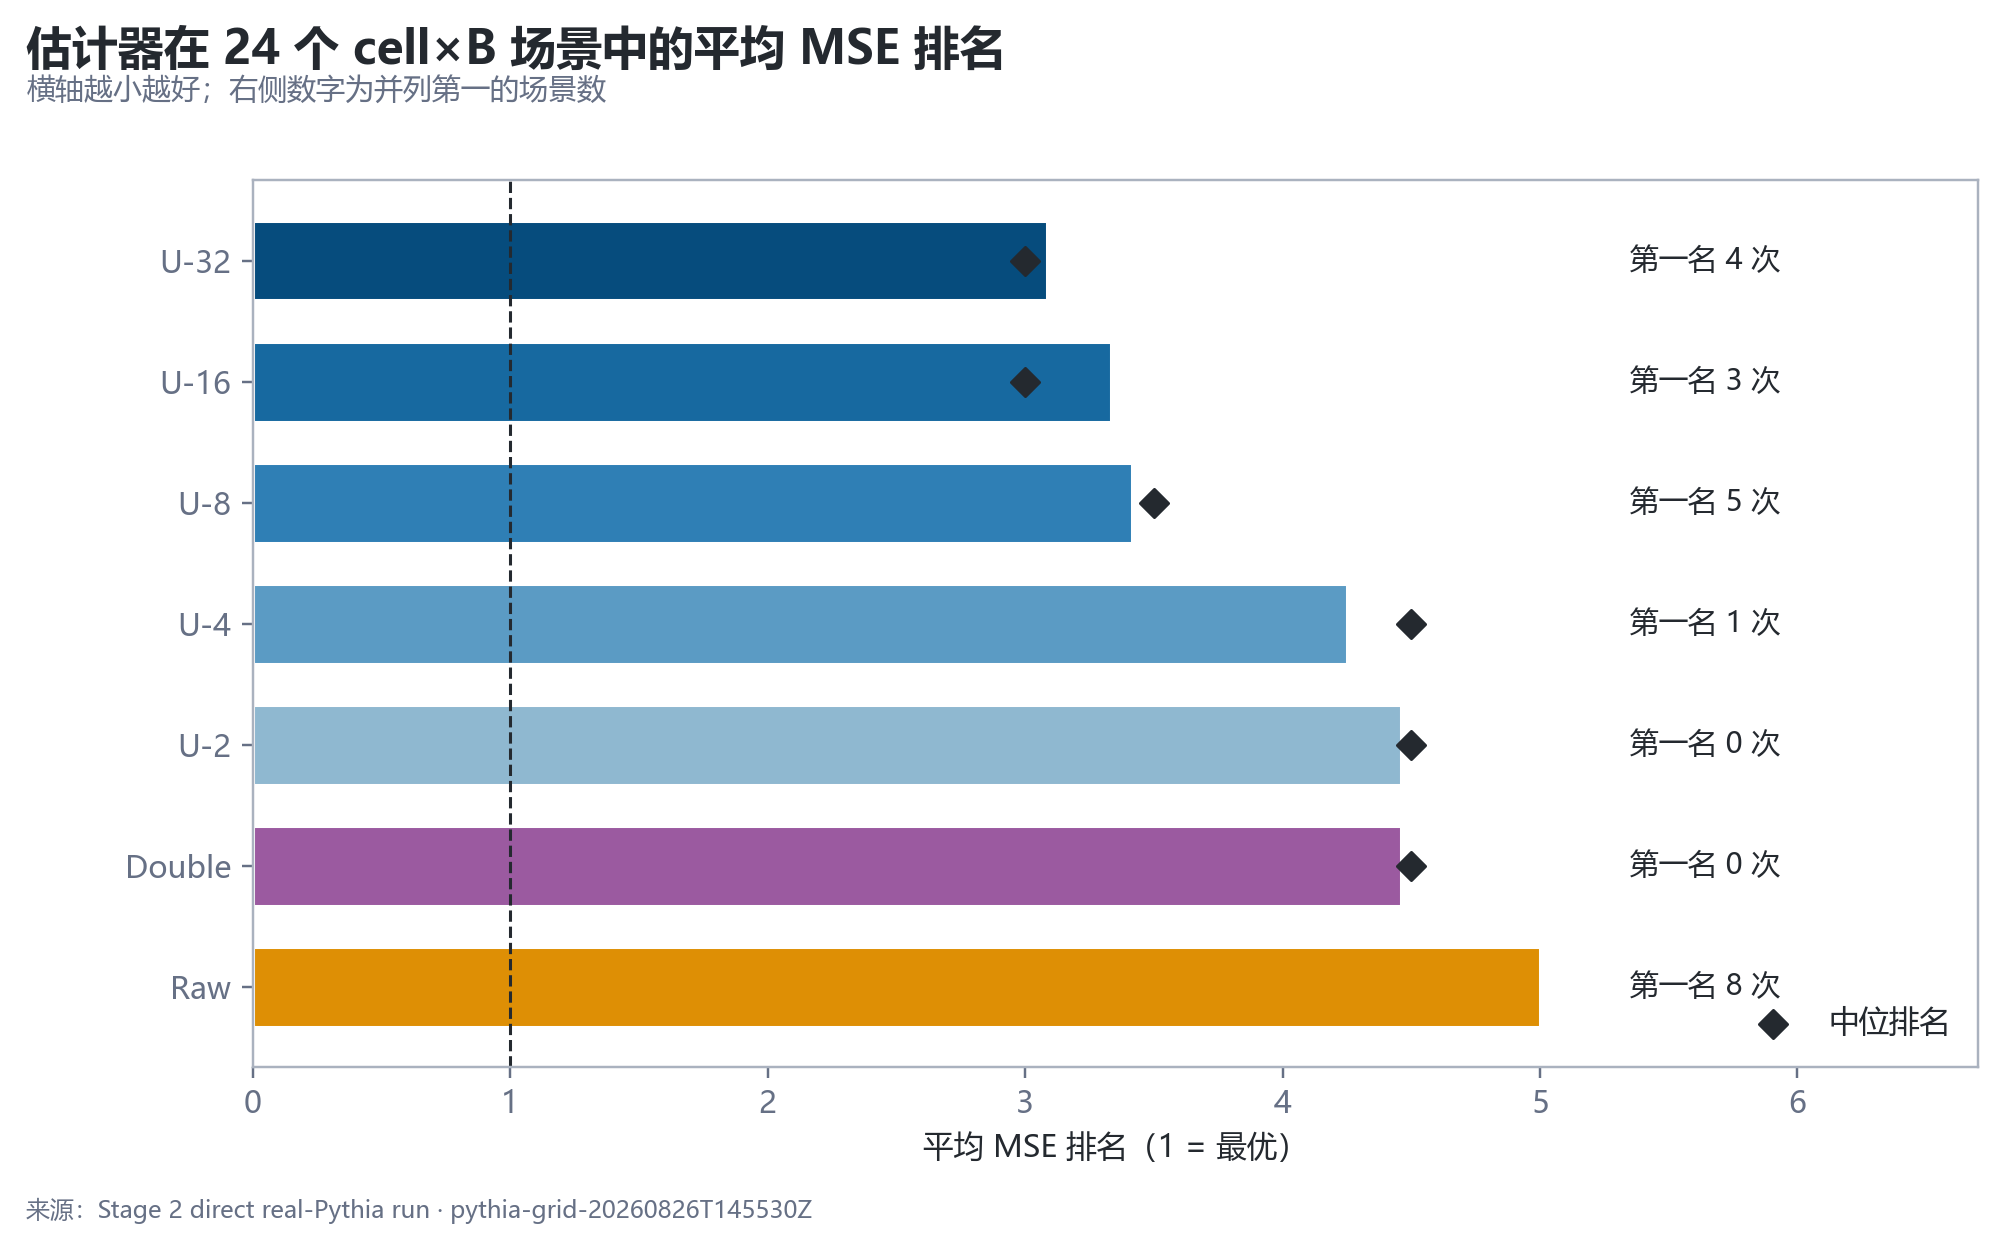
\includegraphics[width=\linewidth]{fig03-method-rank.png}
    \column{0.31\textwidth}
      \begin{block}{24 个 cell$\times B$ 场景}
        \begin{itemize}
          \item U-32：平均 3.08
          \item U-16：平均 3.33
          \item U-8：平均 3.42
          \item Raw：平均 5.00
        \end{itemize}
      \end{block}
      {\small Raw 有 \best{8 次第一}，但中位排名第 7。}
  \end{columns}
  \sourcefoot{黑色菱形表示中位排名；右侧标注第一名次数。}
  \note{U-32 的平均排名优势不大但最稳定。Raw 的特征是“要么非常好、要么很差”：冠军次数最多，却有最差的中位排名。这正是为什么 Raw 应保留作敏感性对照，而不能单独作为默认。}
\end{frame}

\begin{frame}{相对 Raw：U 系列整体降低 MSE}
  \centering
  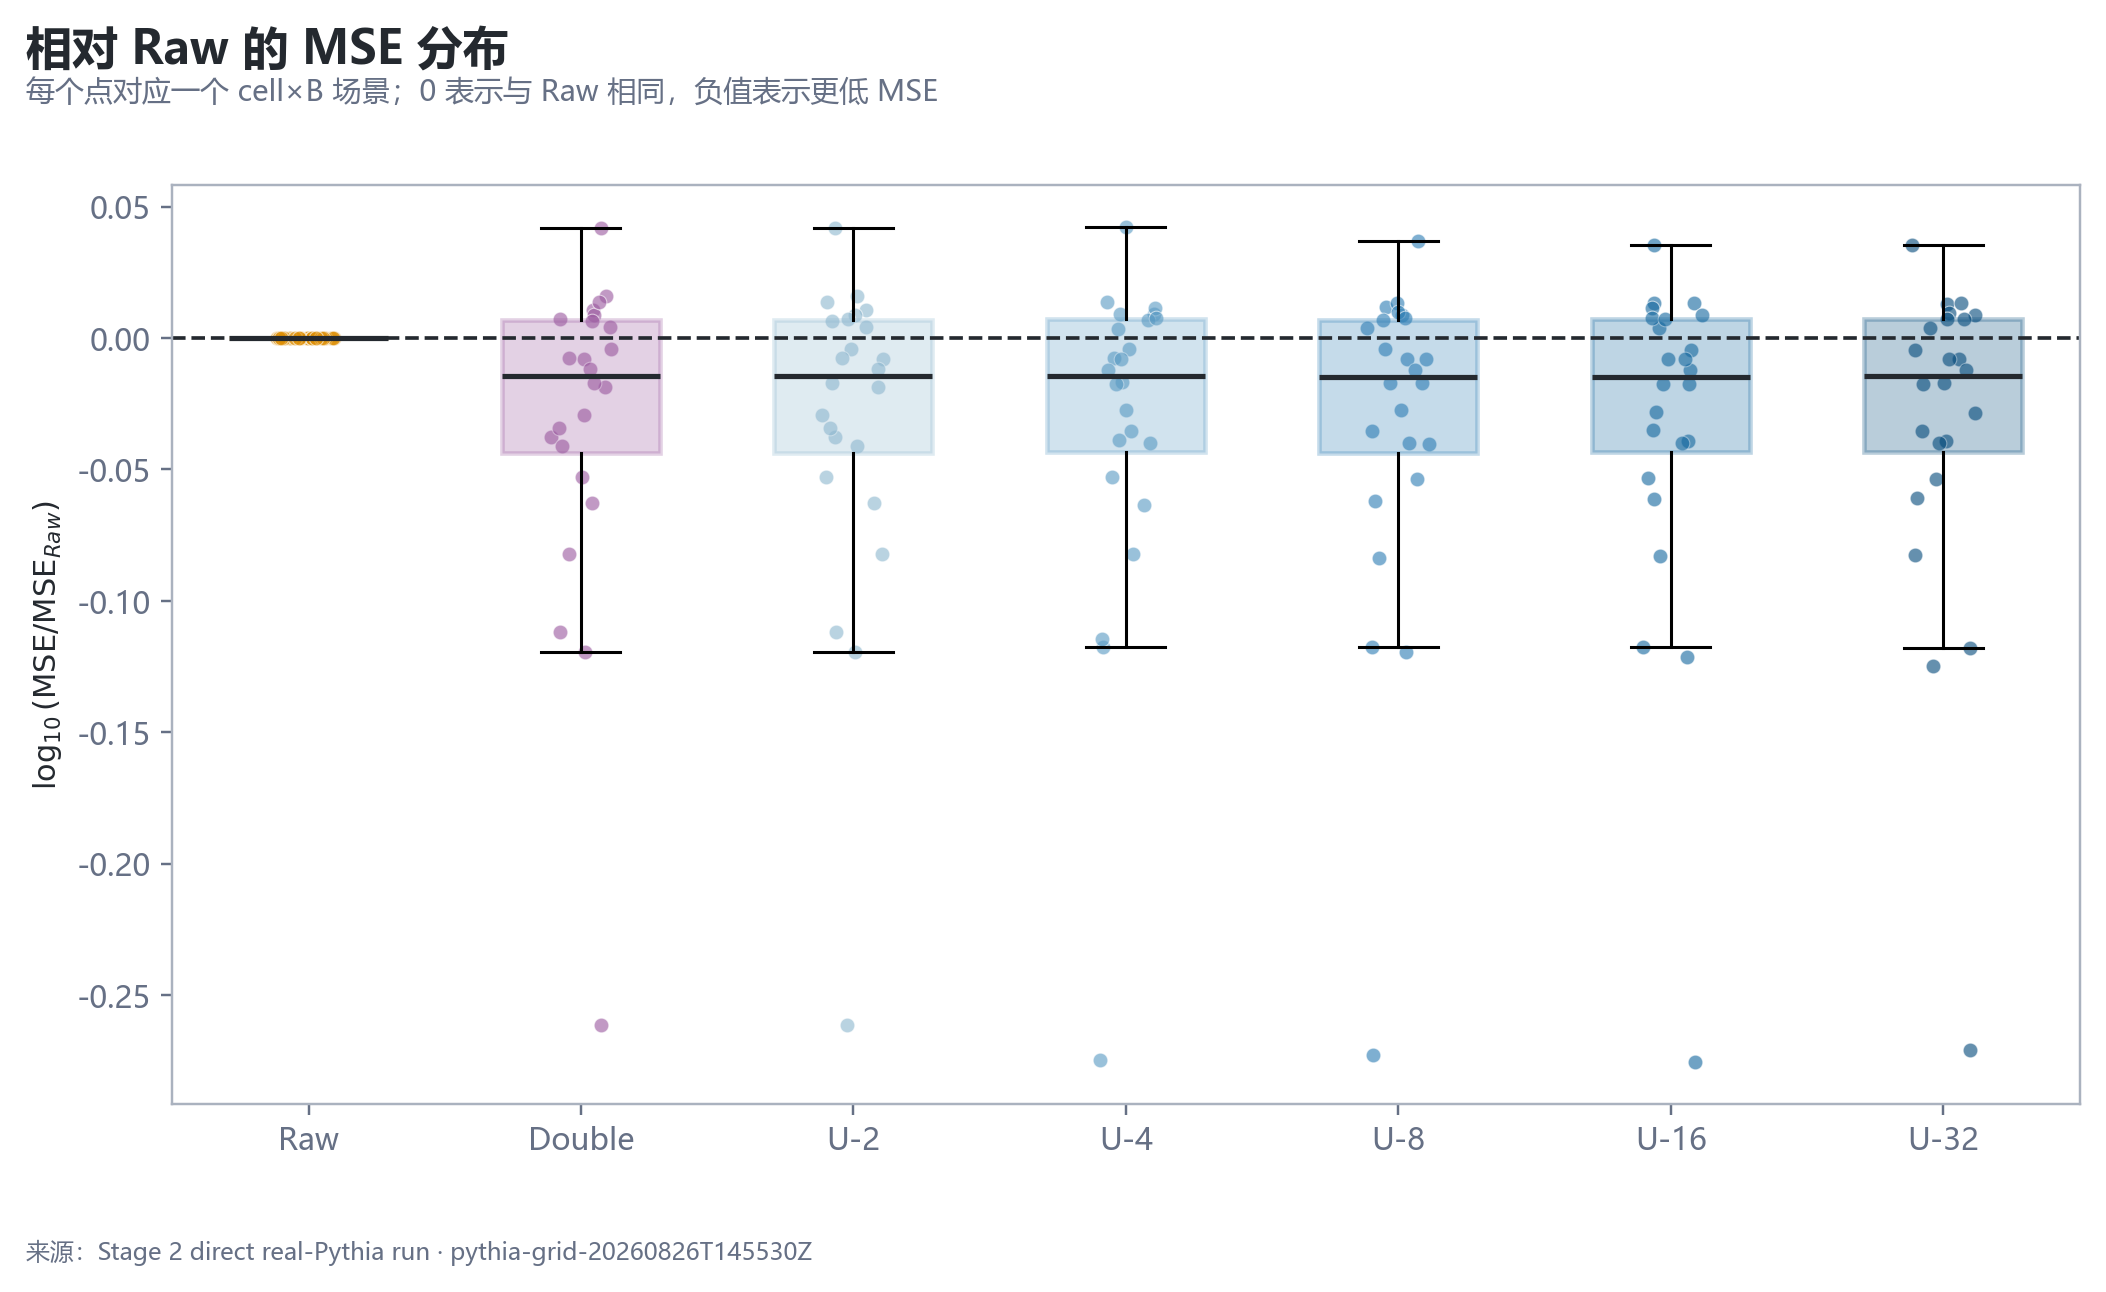
\includegraphics[height=.50\textheight,keepaspectratio]{fig04-relative-mse.png}
  \vspace{-2mm}
  \begin{columns}[T,onlytextwidth]
    \column{.31\textwidth}
      \metriccard{U-32 几何平均 MSE}{-7.59\%}{secondary}
    \column{.31\textwidth}
      \metriccard{中位绝对偏差}{-28.17\%}{good}
    \column{.31\textwidth}
      \metriccard{中位重复方差}{-2.56\%}{accent}
  \end{columns}
  \note{纵轴是相对 Raw 的 log 比例，低于零表示 MSE 更小。U-8、U-16、U-32 的几何平均 MSE 差别只有约万分之一量级，所以最终偏向 U-32 是综合排名，不是声称它在平均误差上大幅击败 U-16。}
\end{frame}

\begin{frame}{阶段依赖之一：Pythia-14M}
  \centering
  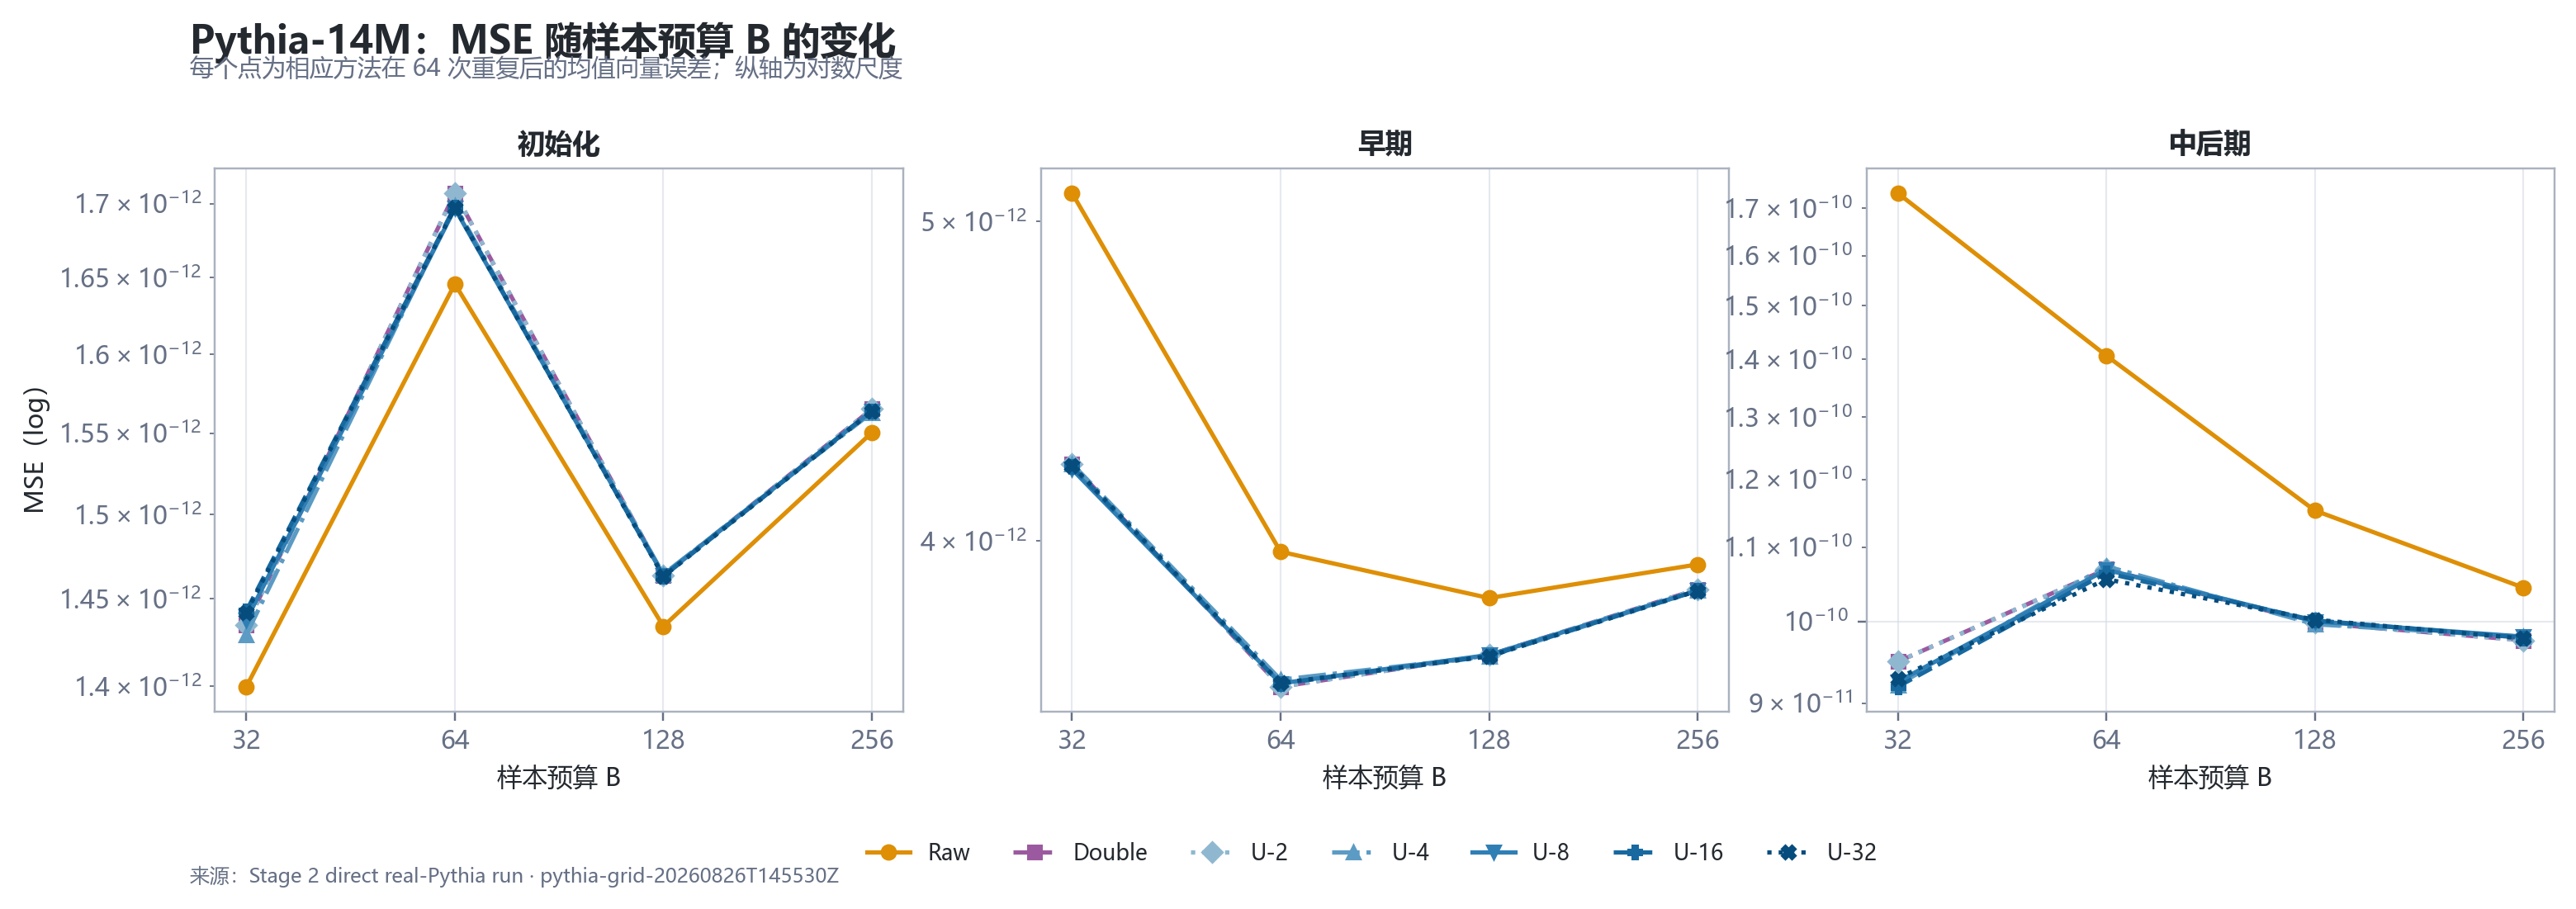
\includegraphics[width=.94\textwidth]{fig05-mse-by-batch-14m.png}
  \begin{beamercolorbox}[rounded=true,sep=.5em,wd=.94\textwidth]{block body}
    \centering
    初始化：Raw、$B=32$\quad|\quad
    早期：Double、$B=64$\quad|\quad
    中后期：U-16、$B=32$
  \end{beamercolorbox}
  \note{14M 展示了阶段切换。尤其 early 是统一 B=32 规则的唯一明显例外：Double、B=64 取得该 cell 的最低观测 MSE。若实验追求跨模型一致性仍选 U-32、B=32；若只做 14M early，可用这个特化点。}
\end{frame}

\begin{frame}{阶段依赖之二：Pythia-31M}
  \centering
  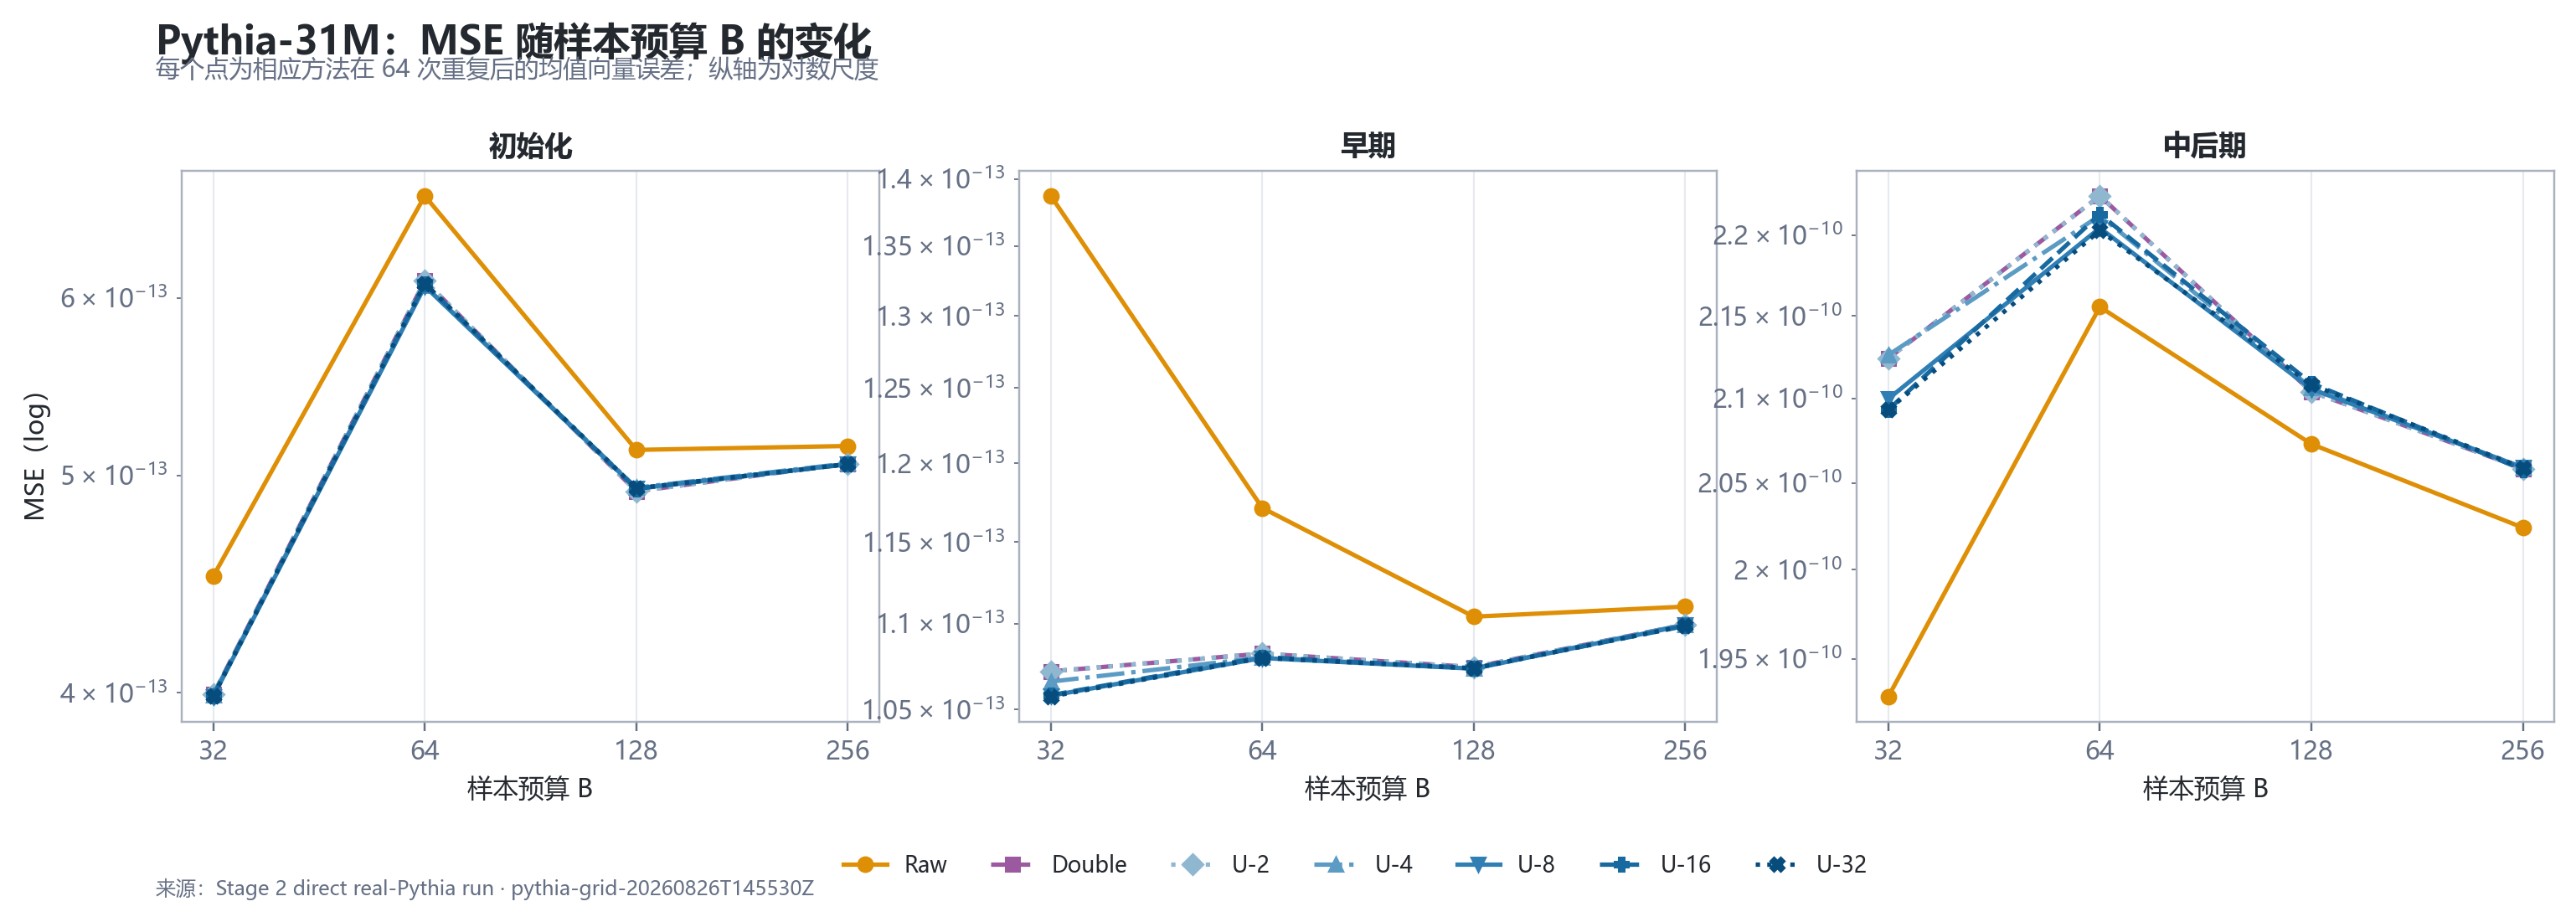
\includegraphics[width=.94\textwidth]{fig06-mse-by-batch-31m.png}
  \begin{beamercolorbox}[rounded=true,sep=.5em,wd=.94\textwidth]{block body}
    \centering
    初始化：U-8、$B=32$\quad|\quad
    早期：U-32、$B=32$\quad|\quad
    中后期：Raw、$B=32$
  \end{beamercolorbox}
  \note{31M 的三个阶段分别由 U-8、U-32、Raw 胜出，说明阶段依赖不是只出现在小模型。中后期 Raw 的胜出也是保留 Raw 对照的直接理由。B=64 的 n=18 格子要谨慎解读，但全局最优仍在 B=32。}
\end{frame}

\begin{frame}{排序保持接近，差异主要来自误差幅度}
  \begin{columns}[T,onlytextwidth]
    \column{0.55\textwidth}
      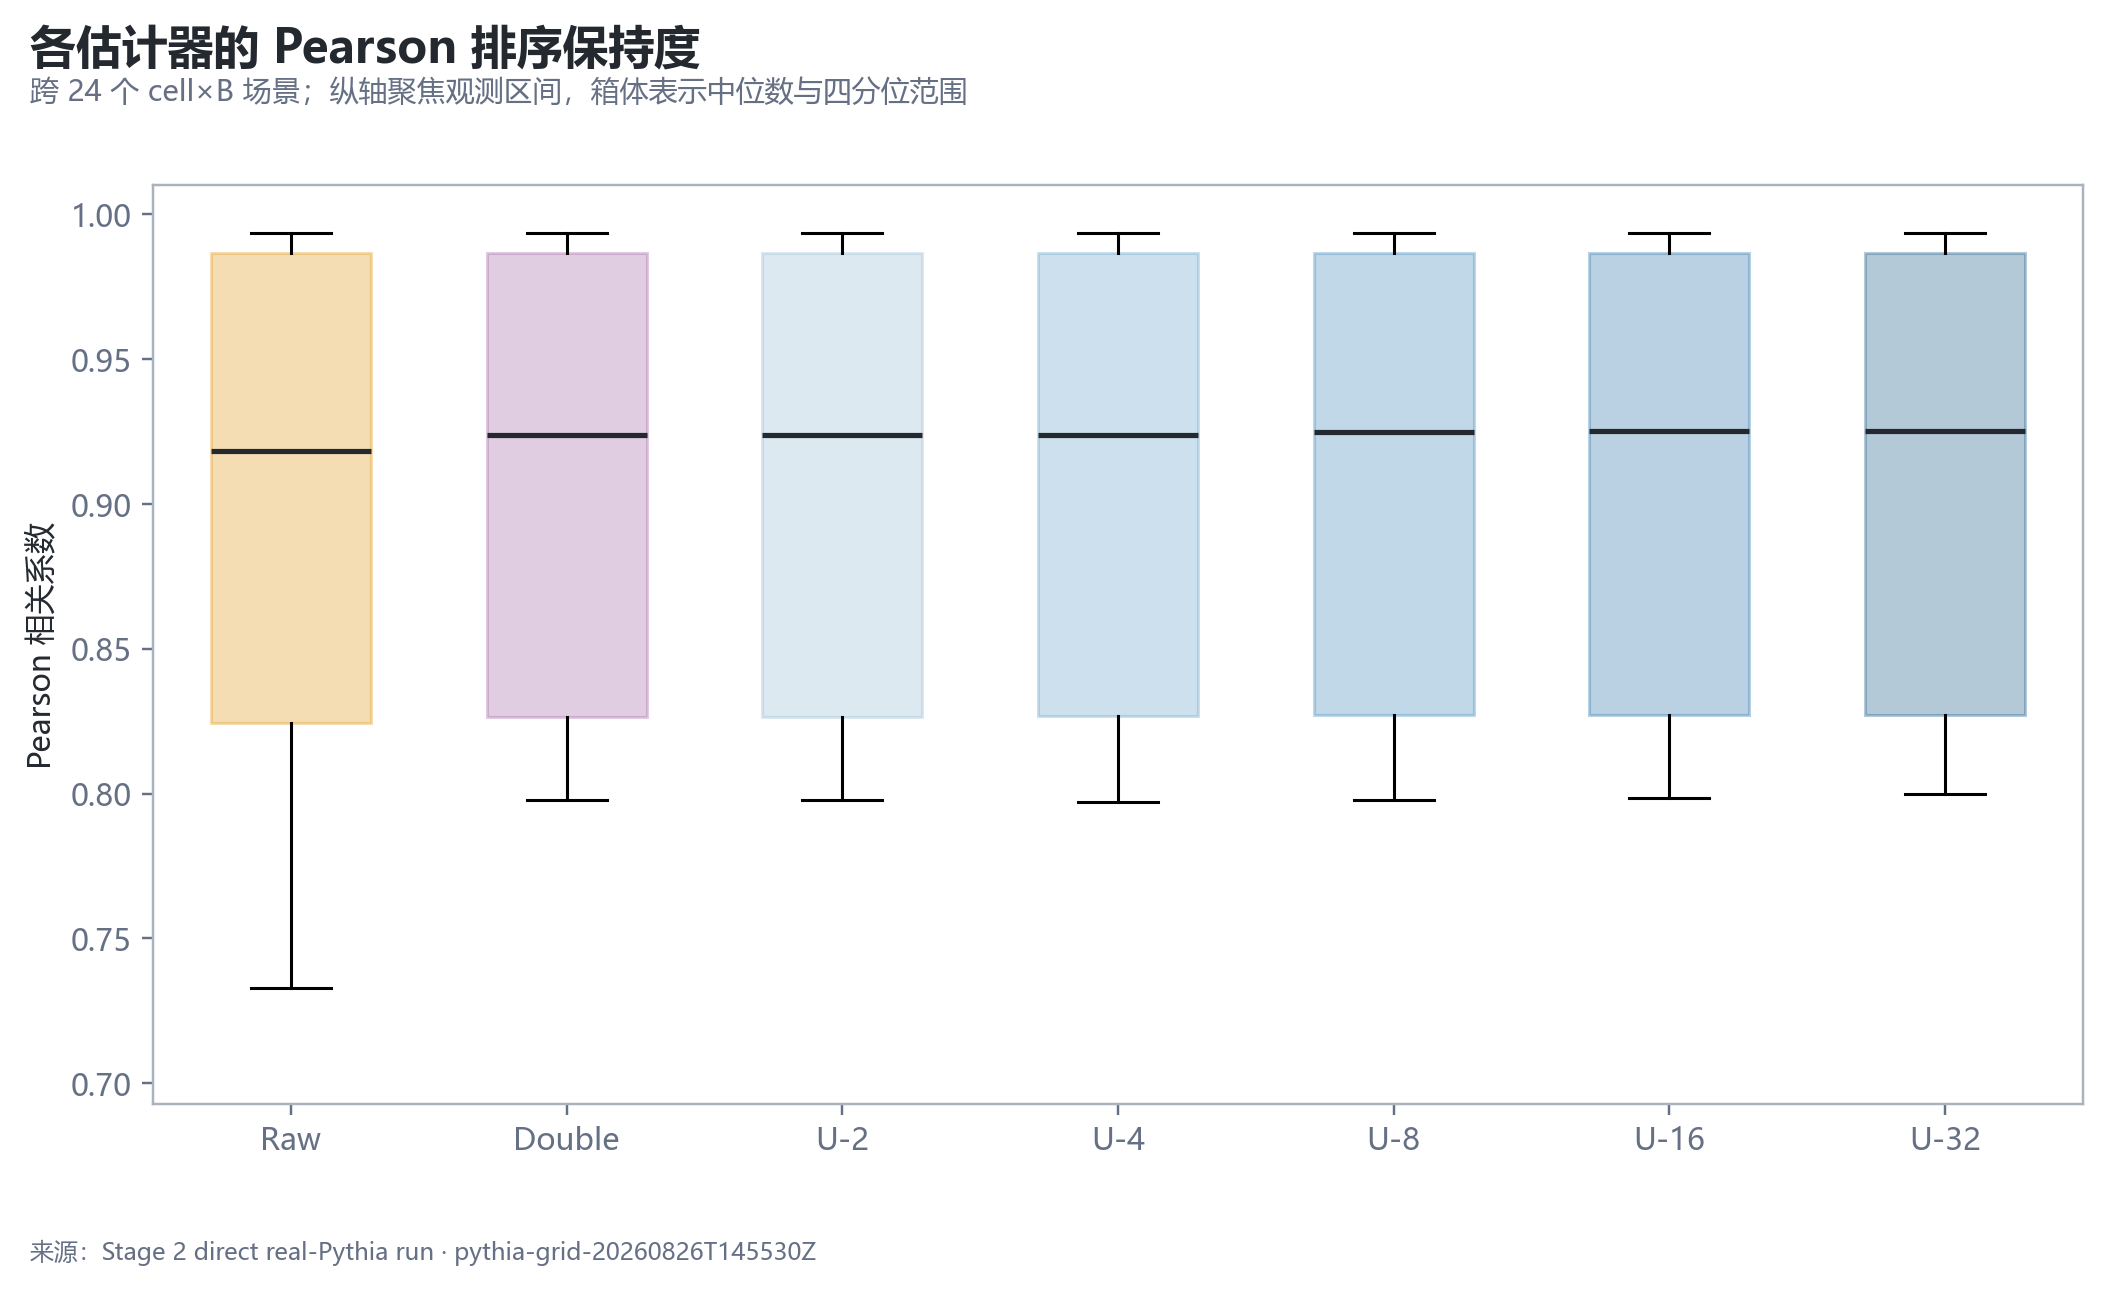
\includegraphics[width=\linewidth]{fig07-pearson-distribution.png}
    \column{0.41\textwidth}
      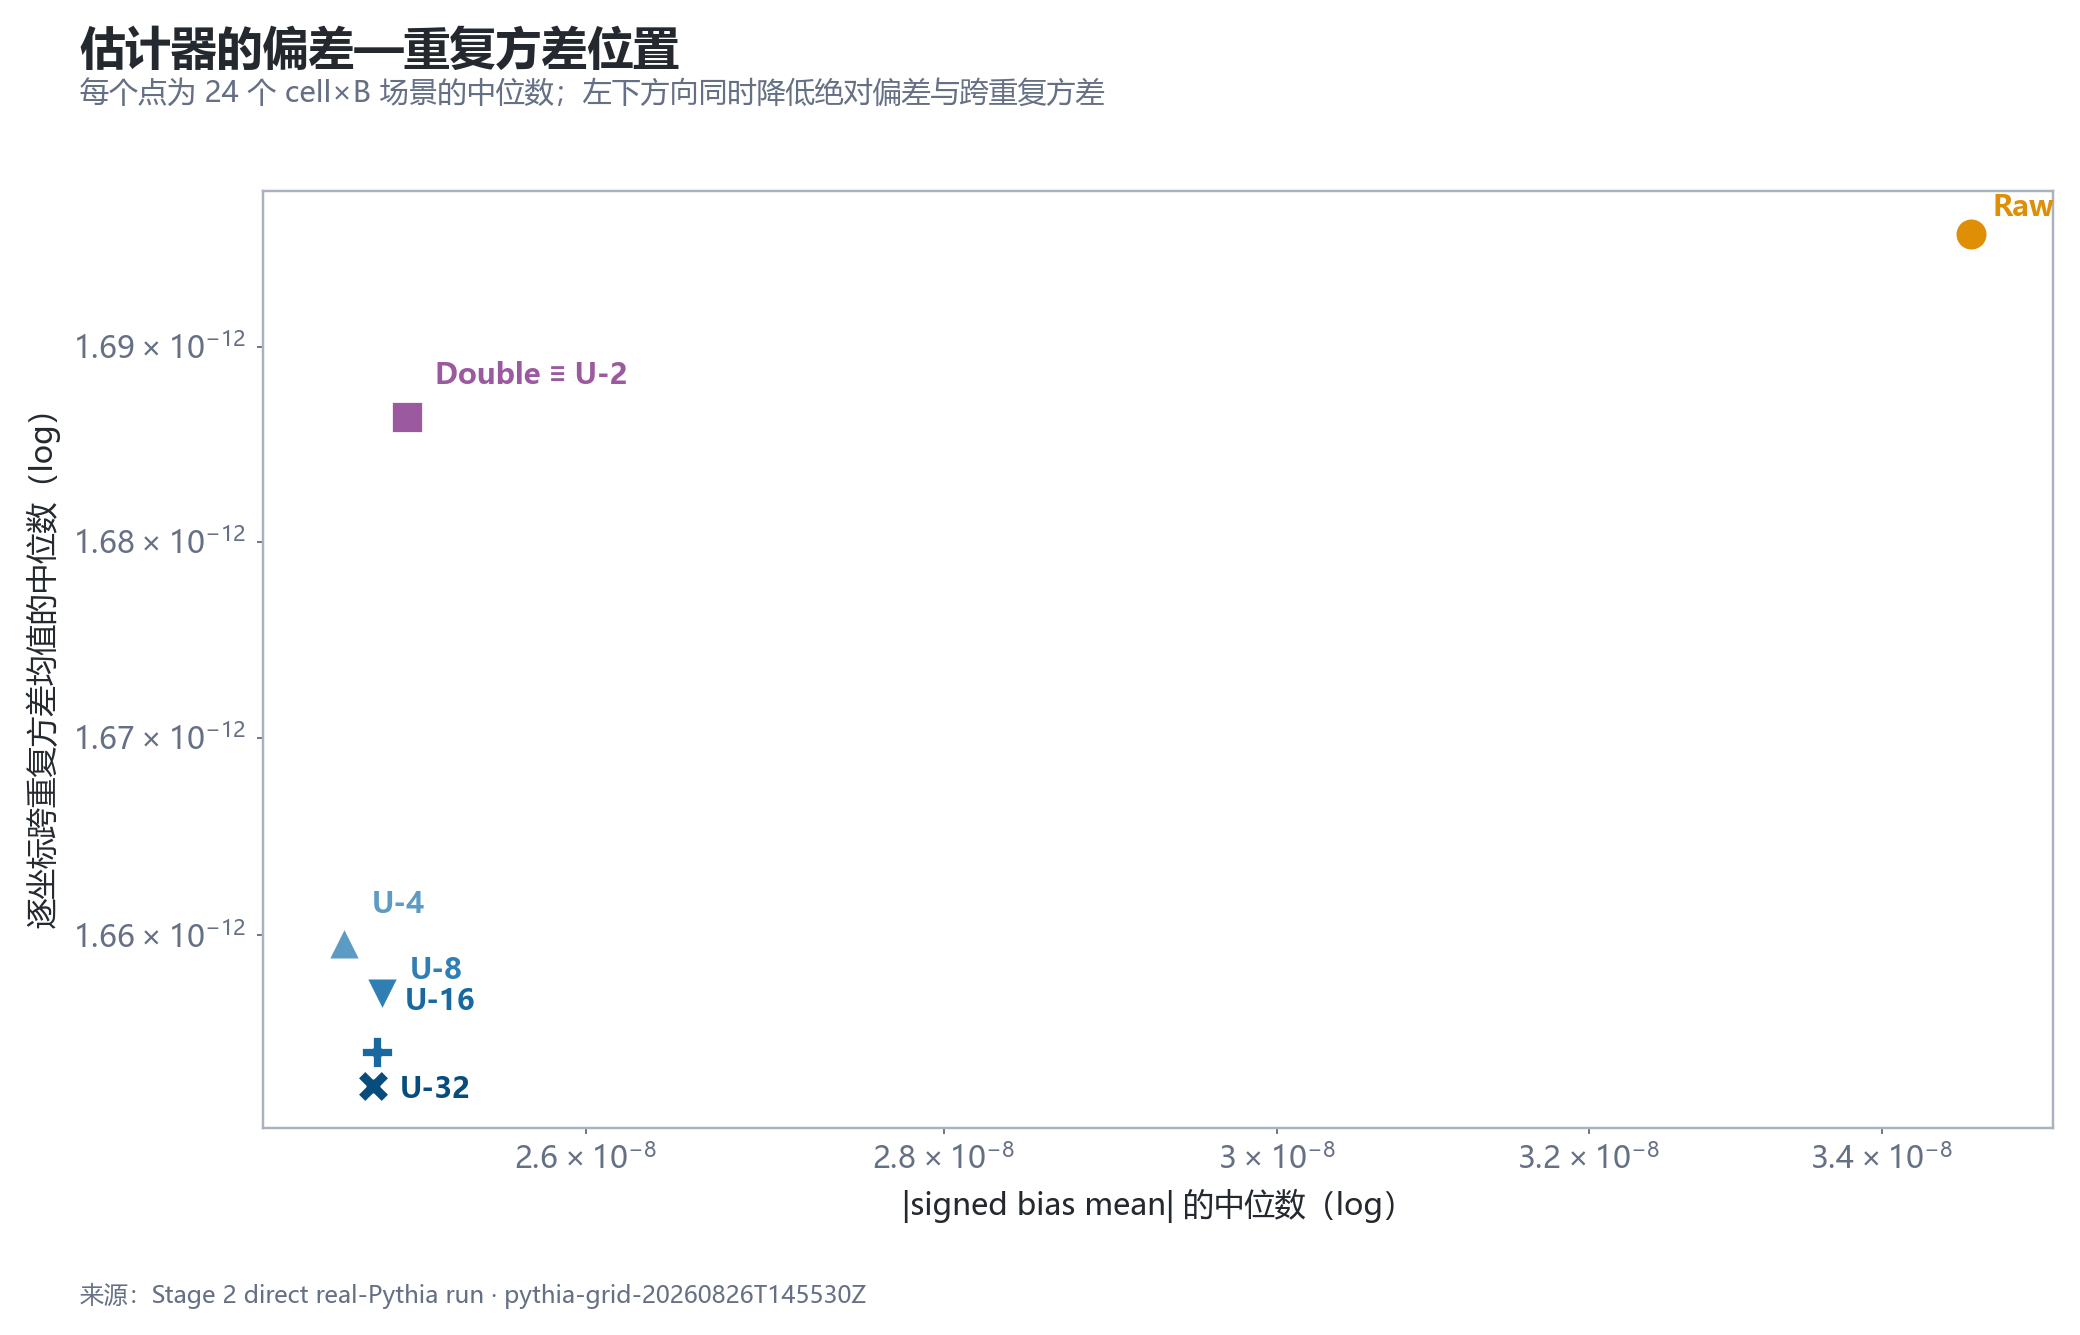
\includegraphics[width=\linewidth]{fig08-bias-variance.png}
  \end{columns}
  \begin{columns}[T,onlytextwidth]
    \column{.50\textwidth}
      {\small Pearson 中位数：U-32 \best{0.9252}，Raw 0.9182}
    \column{.46\textwidth}
      {\small U-32 相对 Raw：偏差与重复方差均下降}
  \end{columns}
  \sourcefoot{Double 与 U-2 完全重合；左图聚焦 Pearson 的主要区间。}
  \note{所有方法的 Pearson 分布高度重合，说明方法选择不会彻底改变排序结构。差异更集中在偏差和 MSE 幅度。右图左下更好，U-32 最接近左下角；Raw 偏差和方差都更高。}
\end{frame}

\begin{frame}{样本预算：更大并不自动更准}
  \begin{columns}[T,onlytextwidth]
    \column{0.66\textwidth}
      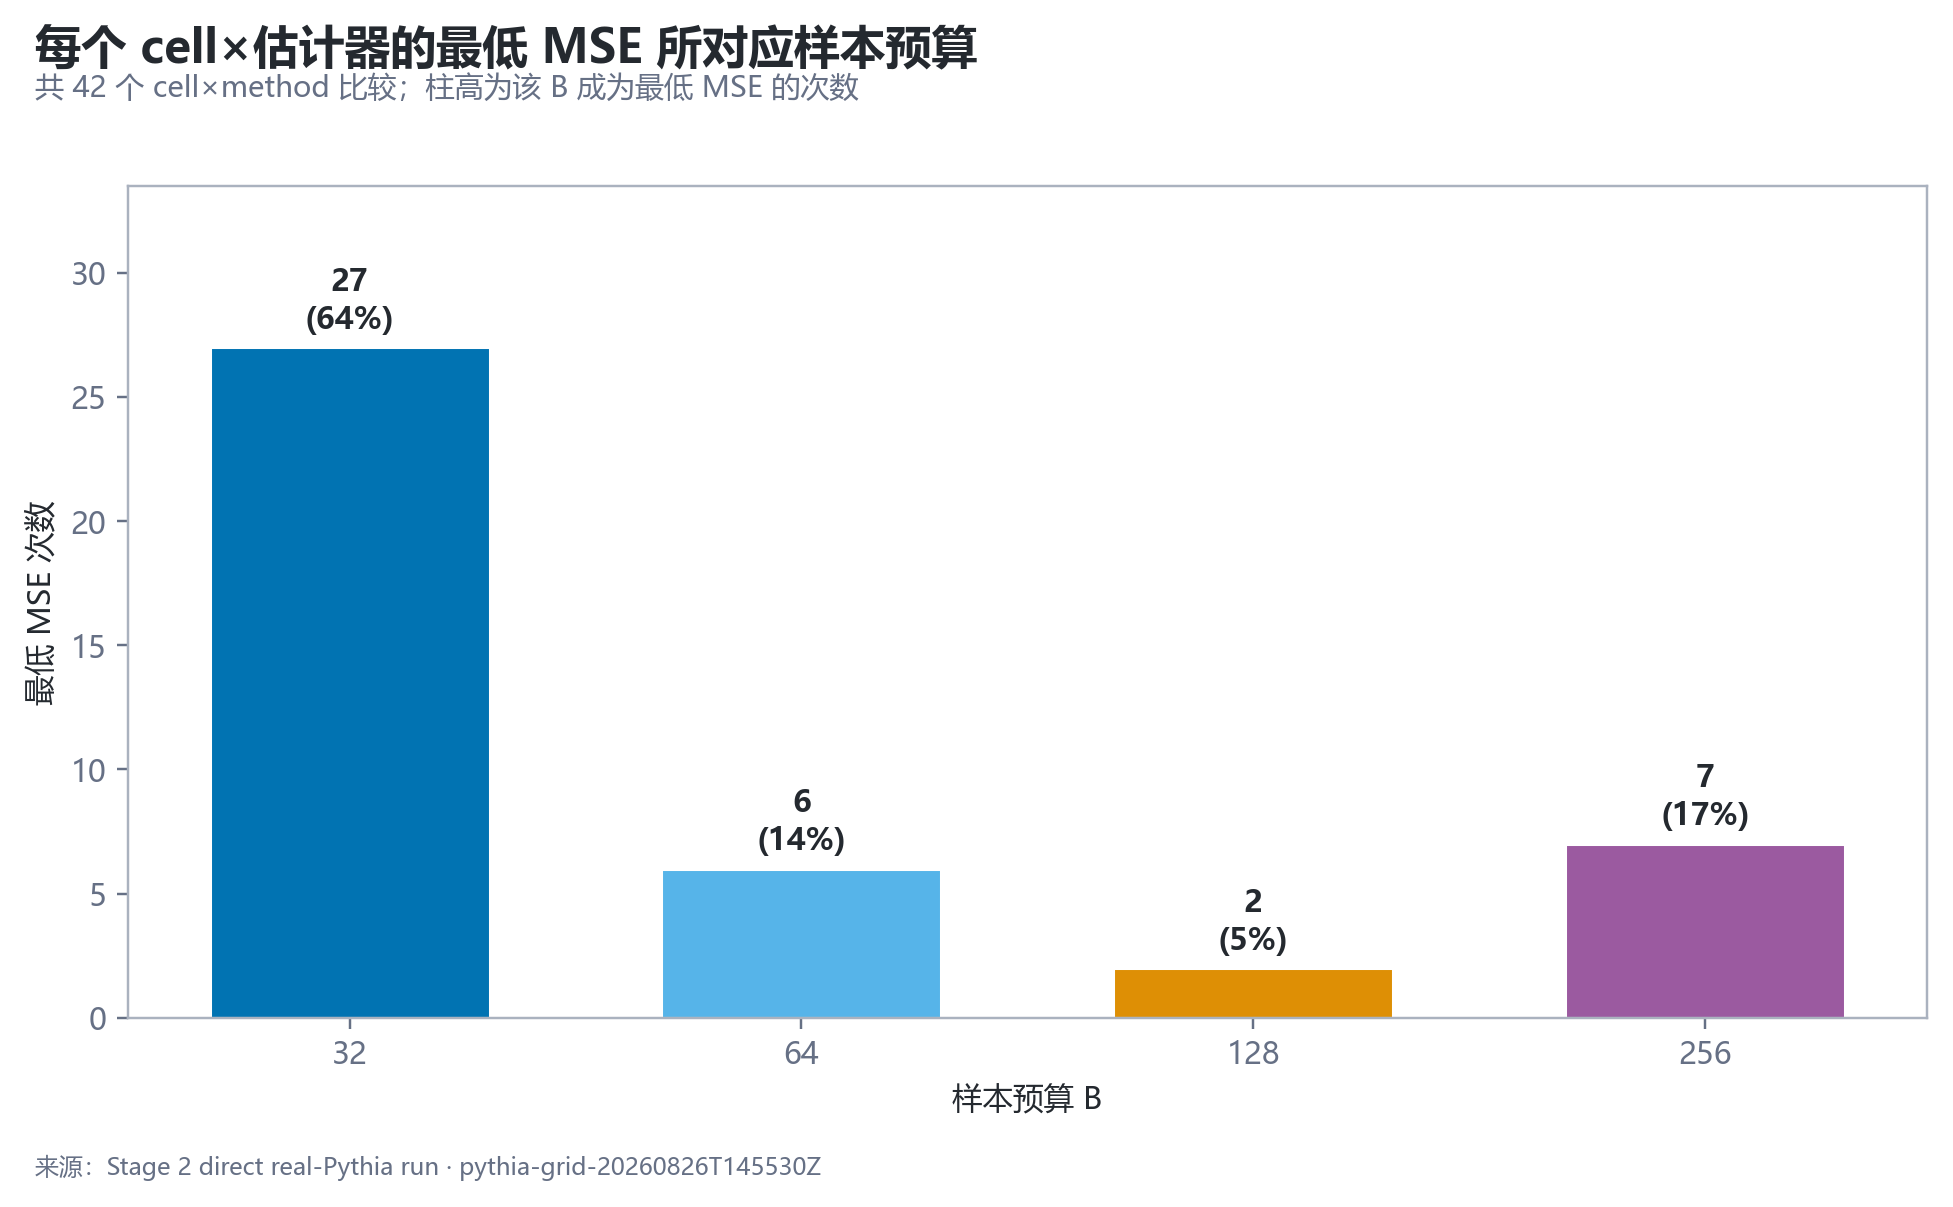
\includegraphics[width=\linewidth]{fig09-best-batch-frequency.png}
    \column{0.30\textwidth}
      \begin{block}{42 个 cell$\times$method}
        \begin{itemize}
          \item \best{$B=32$：27 次}
          \item $B=64$：6 次
          \item $B=128$：2 次
          \item $B=256$：7 次
        \end{itemize}
      \end{block}
      \vspace{1mm}
      {\small\caution{结论：}当前比较中，增大 $B$ 不保证降低 MSE。}
  \end{columns}
  \note{这页直接回答样本预算。B=32 在 64.3\% 的 cell-method 组合中最好。可能原因不是“少样本更有统计效率”，而是当前估计器与参考向量、分组方式共同作用；所以这里做经验决策，不做机制外推。}
\end{frame}

\begin{frame}{成本：时间随 $B$ 上升，显存随模型规模上升}
  \begin{columns}[T,onlytextwidth]
    \column{0.56\textwidth}
      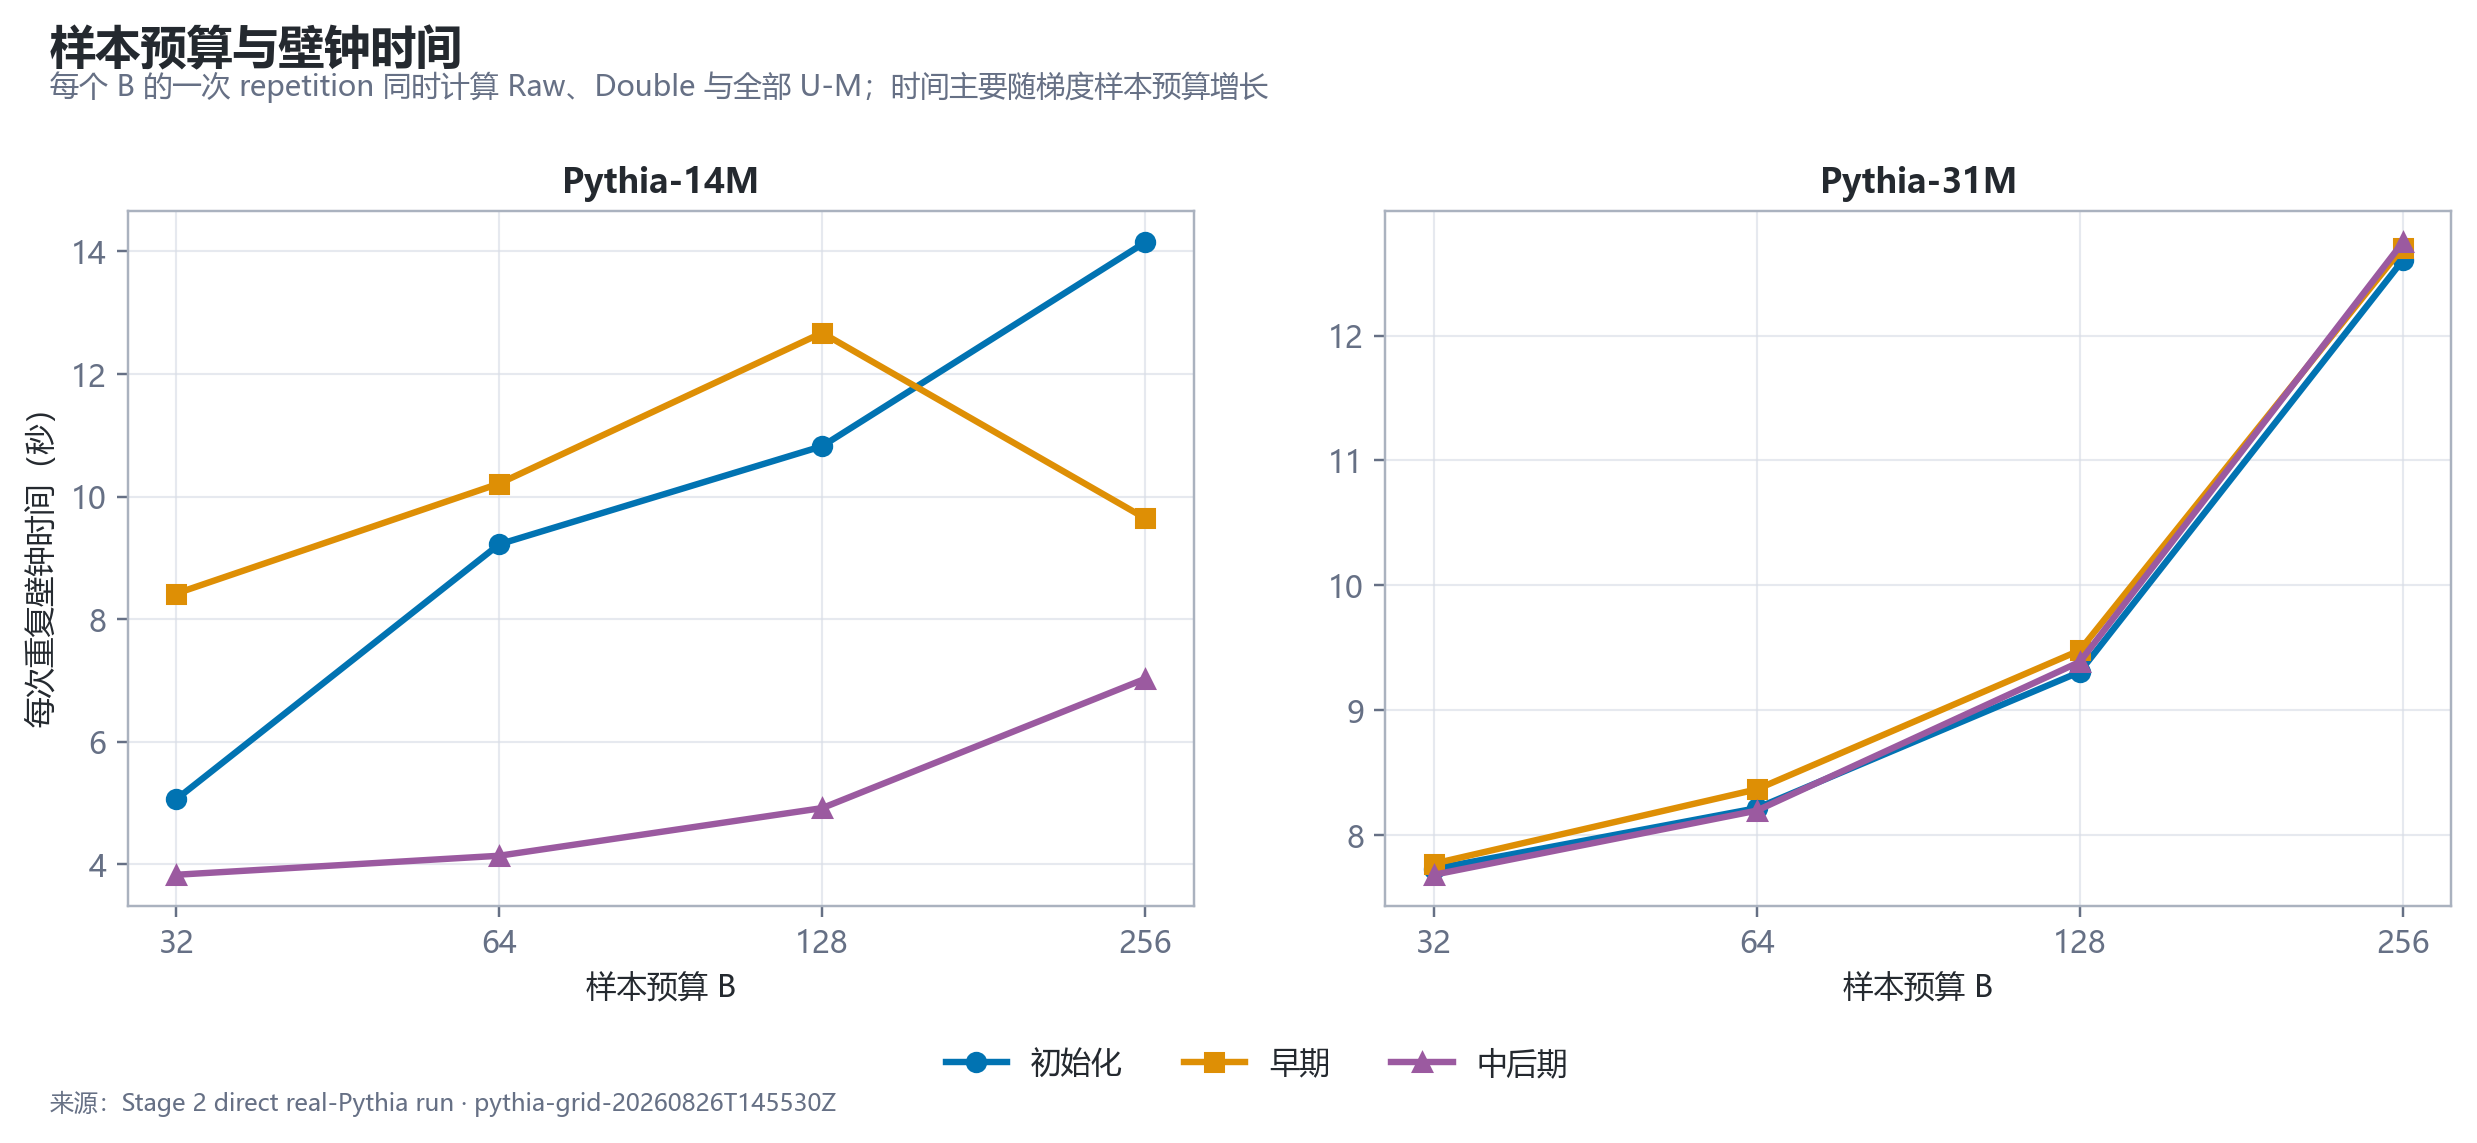
\includegraphics[width=\linewidth]{fig10-runtime-scaling.png}
    \column{0.40\textwidth}
      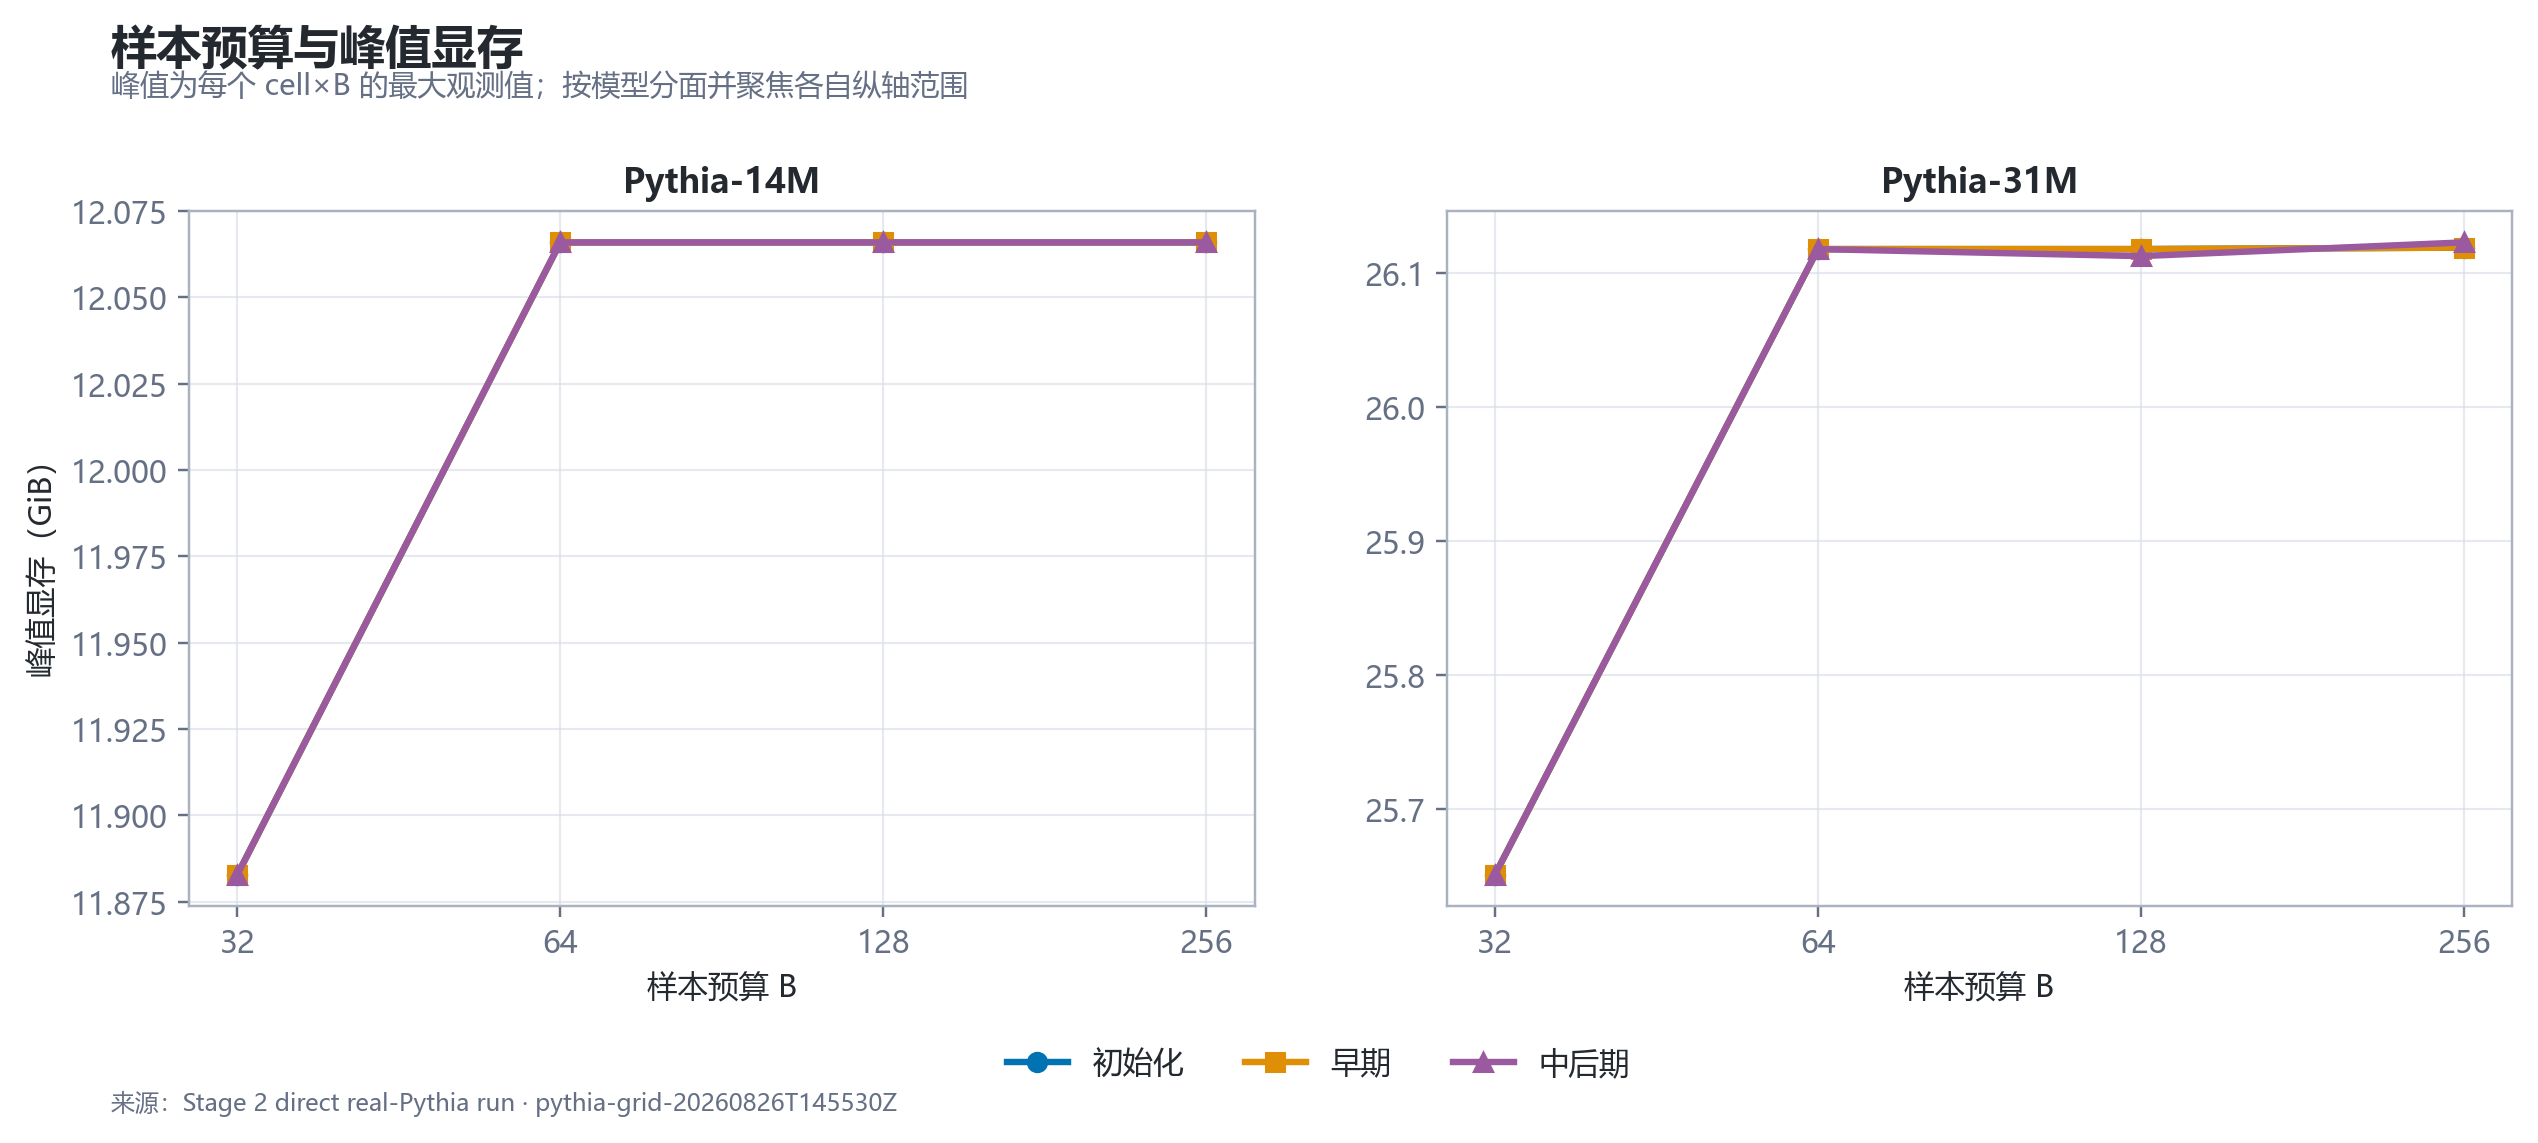
\includegraphics[width=\linewidth]{fig11-memory-scaling.png}
  \end{columns}
  \begin{columns}[T,onlytextwidth]
    \column{.32\textwidth}
      \metriccard{$B=32$ 中位时间}{7.71 s}{secondary}
    \column{.32\textwidth}
      \metriccard{$B=256$ 中位时间}{12.65 s}{accent}
    \column{.32\textwidth}
      \metriccard{时间倍率}{1.64$\times$}{good}
  \end{columns}
  \note{时间曲线整体随 B 增长；14M early 有非单调点，说明共享环境中存在计时波动。峰值显存则基本由模型决定：14M 约 12 GiB，31M 约 26 GiB。注意 profiler 一次计算全部方法，不能用这张图比较某个 estimator 的单独速度。}
\end{frame}

\begin{frame}{精度--成本联合：$B=32$ 是稳健起点}
  \centering
  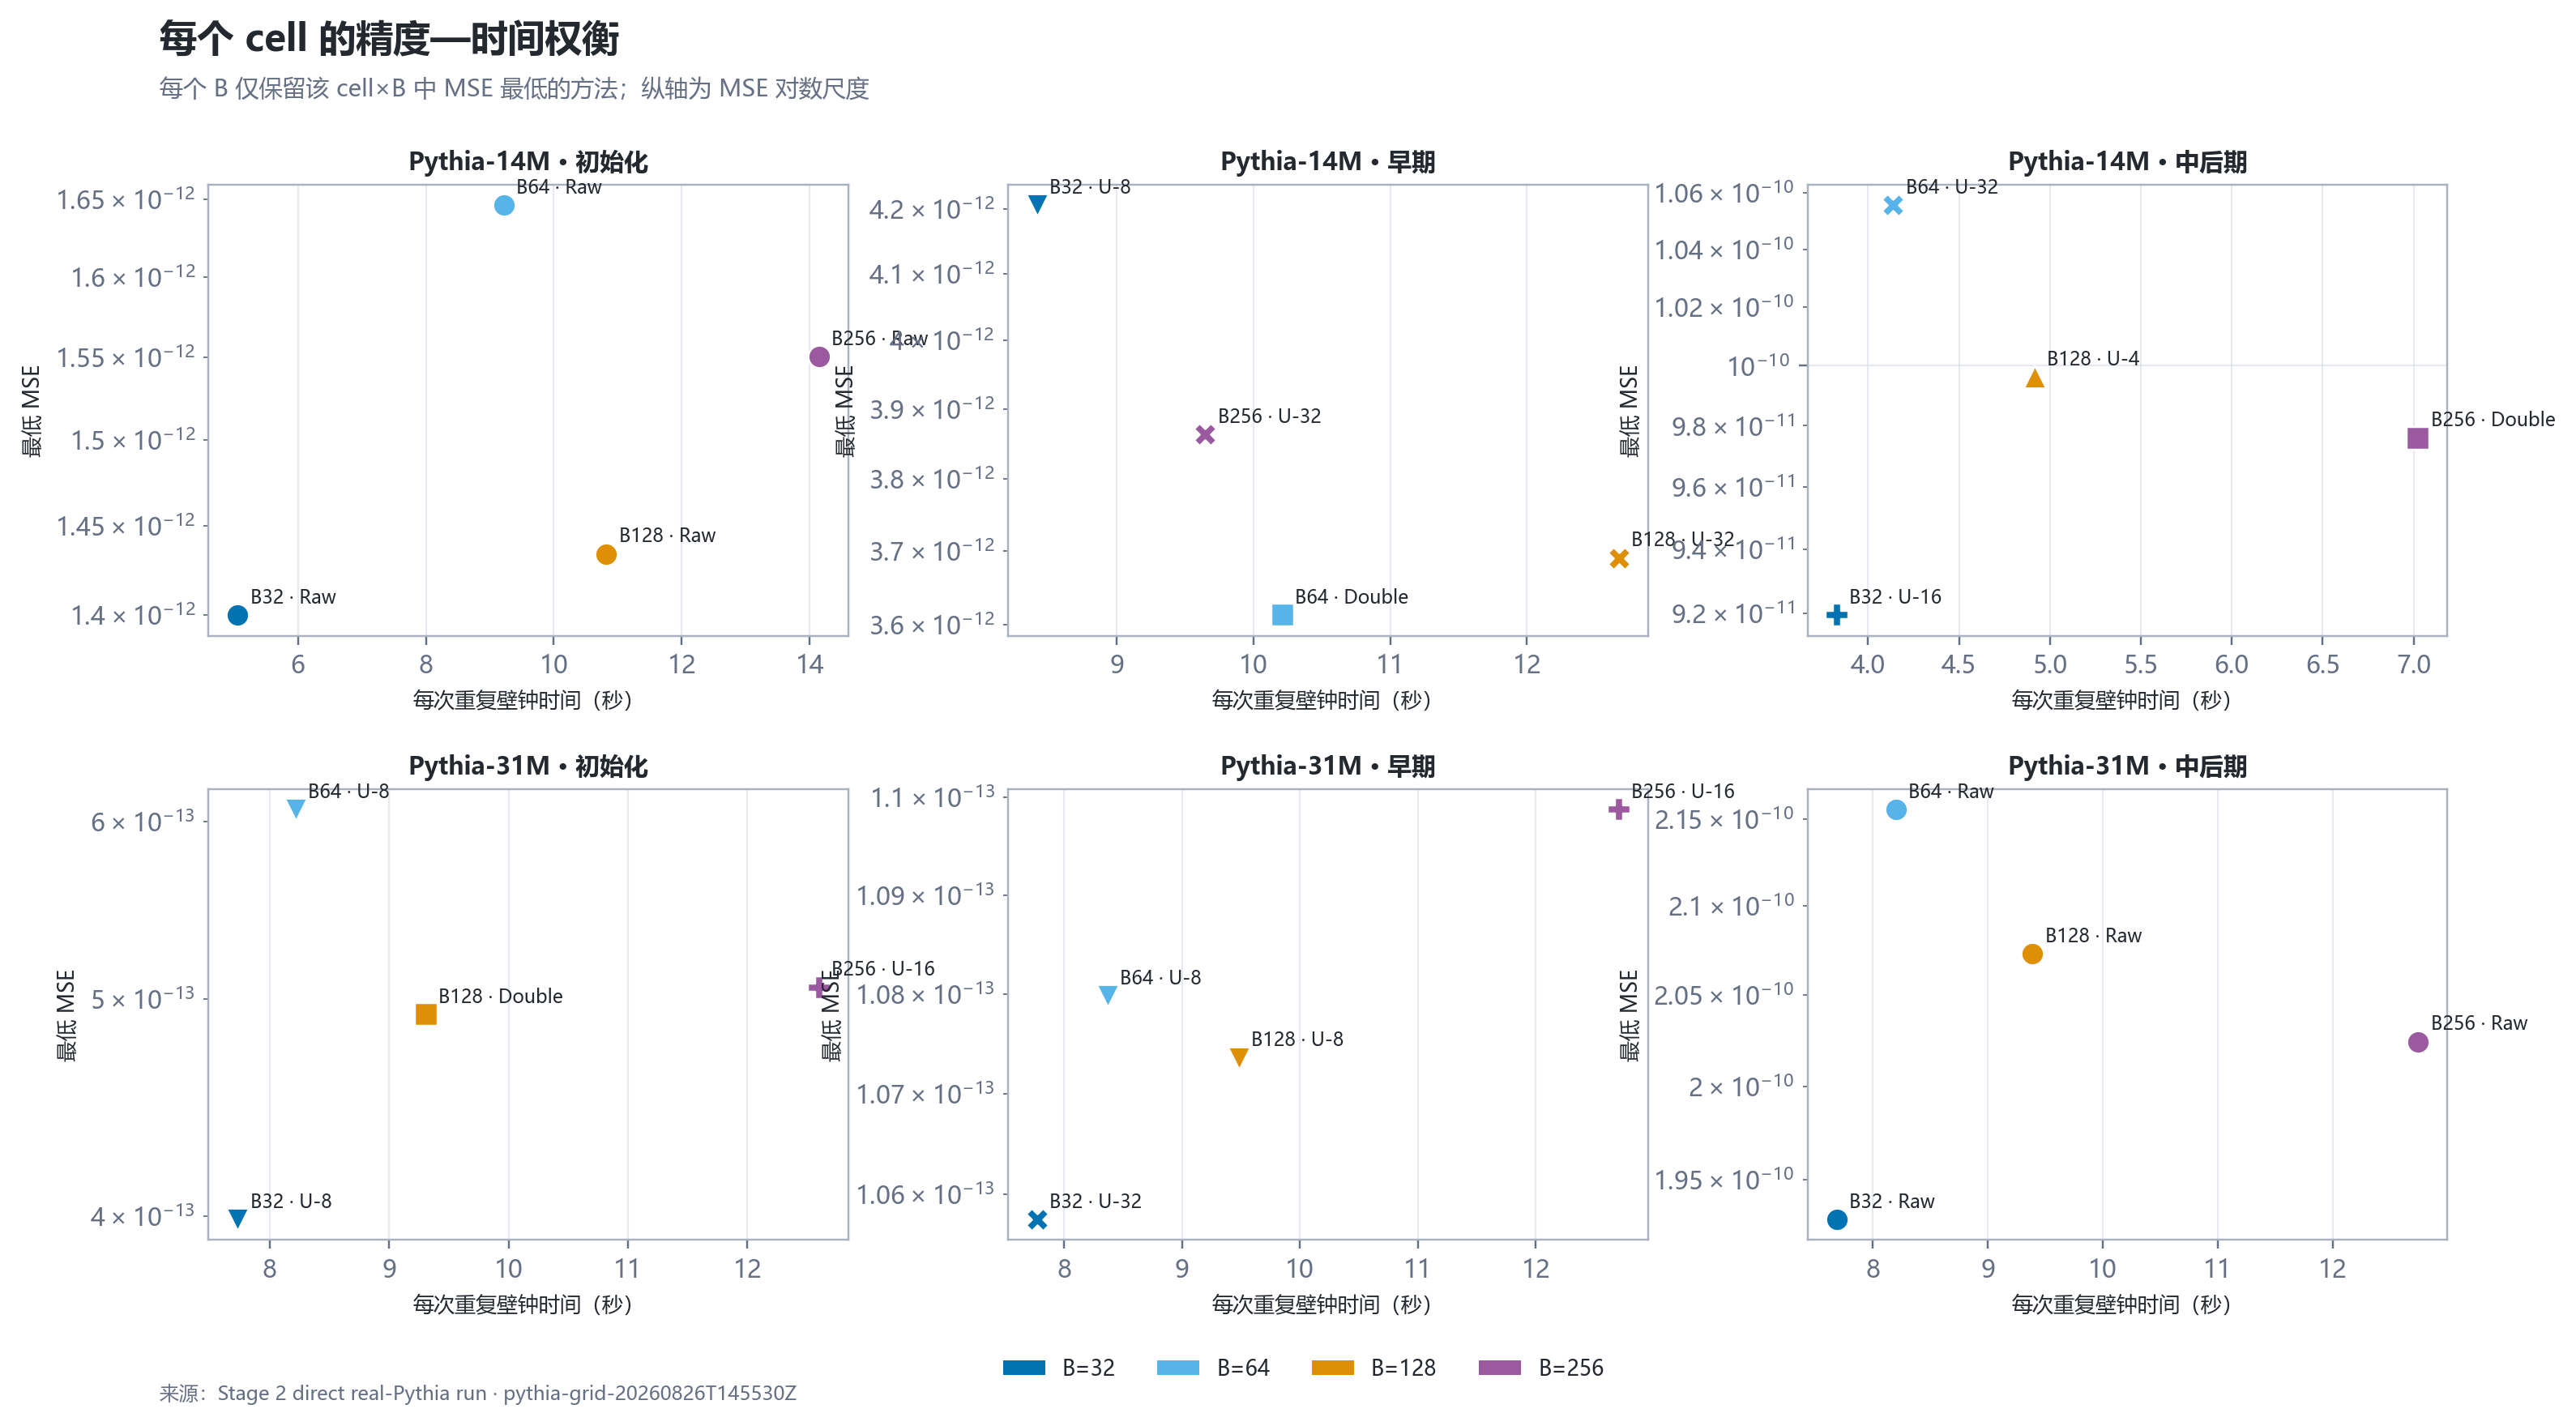
\includegraphics[height=.54\textheight,keepaspectratio]{fig12-accuracy-cost.png}
  \vspace{-1mm}
  \begin{beamercolorbox}[rounded=true,sep=.5em,wd=.92\textwidth]{block body}
    \centering
    6 个 cell 中 \best{5 个全局最低 MSE 位于 $B=32$}；唯一例外为 14M early 的 Double、$B=64$
  \end{beamercolorbox}
  \note{每个小面板只标出同一 B 下 MSE 最低的方法。横轴是 wall time，纵轴是 MSE。多数 cell 的最优点既在最低成本档，又是最低误差；因此 B=32 是精度和时间共同支持的默认点。}
\end{frame}

\begin{frame}{后续实验：按使用情境选，而不是追逐单次冠军}
  \small
  \begin{tabularx}{\textwidth}{>{\raggedright\arraybackslash\bfseries}p{2.3cm}>{\raggedright\arraybackslash}p{2.4cm}>{\centering\arraybackslash}p{1.0cm}X}
    \toprule
    使用情境 & 主估计器 & $B$ & 配套策略 \\
    \midrule
    跨模型统一默认 & \best{U-32} & \best{32} & 保留 Raw；平均排名最佳、成本最低档 \\
    初始化 & \best{U-8} & 32 & 保留 Raw；两模型平均排名更好 \\
    训练早期 & \best{U-32} & 32 & 14M 专项可用 Double、64 \\
    中后期 & \best{U-16 / U-32} & 32 & 保留 Raw；31M 中后期 Raw 胜出 \\
    最小双方法 & U-32 & 32 & 加 Raw，覆盖稳健主线与异质性基线 \\
    三方法输出 & Raw+U-16+U-32 & 32 & 初始化时 U-16 换为 U-8 \\
    \bottomrule
  \end{tabularx}
  \vspace{2mm}
  \begin{beamercolorbox}[rounded=true,sep=.55em]{block body}
    \centering
    Double 与 U-2 只保留一个；U-4 主要用于消融。
  \end{beamercolorbox}
  \note{这是可以直接抄到下一轮实验配置里的决策表。最小方案只跑 U-32 和 Raw；预算允许时再加 U-16。初始化专项把 U-16 换成 U-8。Double 与 U-2 的重复输出没有信息增益。}
\end{frame}

\begin{frame}{逐 cell 的观测精度：量级与相关性}
  \small
  \centering
  \begin{tabular}{llrrrr}
    \toprule
    模型--阶段 & 方法 & $B$ & MSE & MAE & Pearson \\
    \midrule
    14M--初始化 & Raw & 32 & $1.40{\times}10^{-12}$ & $5.88{\times}10^{-8}$ & .9870 \\
    14M--早期 & Double & 64 & $3.61{\times}10^{-12}$ & $1.30{\times}10^{-7}$ & .9445 \\
    14M--中后期 & U-16 & 32 & $9.19{\times}10^{-11}$ & $1.85{\times}10^{-7}$ & .8232 \\
    31M--初始化 & U-8 & 32 & $3.99{\times}10^{-13}$ & $4.84{\times}10^{-8}$ & .9930 \\
    31M--早期 & U-32 & 32 & $1.06{\times}10^{-13}$ & $3.20{\times}10^{-8}$ & .8282 \\
    31M--中后期 & Raw & 32 & $1.93{\times}10^{-10}$ & $2.63{\times}10^{-7}$ & .8982 \\
    \bottomrule
  \end{tabular}
  \vspace{3mm}
  \begin{columns}[T,onlytextwidth]
    \column{.48\textwidth}
      \begin{block}{精度范围}
        MSE：$1.06{\times}10^{-13}$ 至 $1.93{\times}10^{-10}$
      \end{block}
    \column{.48\textwidth}
      \begin{block}{相关性范围}
        Pearson：0.823 至 0.993
      \end{block}
  \end{columns}
  \note{这页给出可直接引用的数值。不要跨 cell 比较 MSE 的绝对值来判断阶段难度，因为参考向量尺度不同；同一 cell 内的方法和 B 比较才是本报告的主要精度依据。}
\end{frame}

\begin{frame}{带走四句话}
  \begin{enumerate}
    \setlength{\itemsep}{7mm}
    \item \best{统一默认：U-32、$B=32$。}
    \item \keypoint{阶段化：初始化 U-8；中后期 U-16/U-32；始终保留 Raw。}
    \item \caution{Raw 高异质：冠军次数多，但跨场景中位排名最差。}
    \item Double $\equiv$ U-2；大 $B$ 不保证更准，且成本更高。
  \end{enumerate}
  \vspace{2mm}
  \begin{beamercolorbox}[rounded=true,sep=.8em]{block body}
    \centering
    这批数据支持的是\textbf{可执行的 estimator selection}，而不是“一个方法统治所有阶段”。
  \end{beamercolorbox}
  \note{收束回到开头。统一默认解决工程可执行性；阶段例外保留数据里真实存在的异质性。若听众只记得一行，就是 U-32/B=32 主线，加 Raw 敏感性对照。}
\end{frame}

\begin{frame}{参考文献}
  \footnotesize
  \begin{thebibliography}{9}
    \bibitem{hoeffding}
      W. Hoeffding.
      \newblock A Class of Statistics with Asymptotically Normal Distribution.
      \newblock \emph{The Annals of Mathematical Statistics}, 19(3), 1948.

    \bibitem{pythia}
      S. Biderman et al.
      \newblock Pythia: A Suite for Analyzing Large Language Models Across Training and Scaling.
      \newblock \emph{Proceedings of ICML}, 2023.

    \bibitem{importance}
      P. Molchanov et al.
      \newblock Importance Estimation for Neural Network Pruning.
      \newblock \emph{Proceedings of CVPR}, 2019.

    \bibitem{artifact}
      Parameter Importance Project.
      \newblock Stage 2 direct real-Pythia run:
      \texttt{pythia-grid-20260826T145530Z}.
      \newblock Internal experiment artifact, 2026.
  \end{thebibliography}
  \note{参考文献页只需停留十几秒。前三项提供 U-statistic、Pythia 模型和参数重要性背景；所有具体数字来自最后一项内部运行产物。}
\end{frame}

\begin{frame}[plain]
  \begin{tikzpicture}[remember picture,overlay]
    \fill[primary] (current page.south west) rectangle (current page.north east);
    \draw[secondary,line width=6pt] ([yshift=.9cm]current page.south west)
      -- ([yshift=.9cm]current page.south east);
  \end{tikzpicture}
  \vfill
  \centering
  {\color{white}\Huge\bfseries 谢谢}\\[5mm]
  {\color{white!85}\Large Q\&A}\\[13mm]
  \begin{beamercolorbox}[rounded=true,sep=.8em,wd=.62\textwidth]{block body}
    \centering
    默认：\best{U-32、$B=32$}\\
    对照：Raw
  \end{beamercolorbox}
  \vfill
  {\color{white!65}\small 完整报告、CSV、图表和分析脚本随 slides 一并交付}
  \note{邀请问题。若被问“最终到底跑哪两个”，直接回答 U-32 与 Raw，B=32；然后根据阶段决定是否把 U-16 或 U-8 加回。}
\end{frame}

\appendix

\begin{frame}[plain]
  \begin{tikzpicture}[remember picture,overlay]
    \fill[ink] (current page.south west) rectangle (current page.north east);
    \fill[secondary] (current page.south west)
      rectangle ([xshift=1.25cm]current page.north west);
  \end{tikzpicture}
  \vfill
  \centering
  {\color{white}\Huge\bfseries 附录}\\[3mm]
  {\color{white!70}\large 方法明细、逐 cell 数值与数据身份}
  \vfill
\end{frame}

\begin{frame}{附录 A：完整方法汇总}
  \small
  \centering
  \begin{tabular}{lrrrr}
    \toprule
    方法 & 平均排名 & 中位排名 & 第一名次数 & 几何平均 MSE / Raw \\
    \midrule
    U-32 & \best{3.08} & 3 & 4 & \best{0.9241} \\
    U-16 & 3.33 & 3 & 3 & 0.9242 \\
    U-8 & 3.42 & 3 & 5 & 0.9243 \\
    U-4 & 4.25 & 4 & 1 & 0.9252 \\
    Double & 4.46 & 4.5 & 0 & 0.9269 \\
    U-2 & 4.46 & 4.5 & 0 & 0.9269 \\
    Raw & 5.00 & 7 & \best{8} & 1.0000 \\
    \bottomrule
  \end{tabular}
  \vspace{4mm}
  \begin{beamercolorbox}[rounded=true,sep=.7em,wd=.88\textwidth]{block body}
    U-8 / U-16 / U-32 的几何平均 MSE 彼此只差约 0.02\%，
    因此选择要同时看排名稳定性与阶段适用性。
  \end{beamercolorbox}
\end{frame}

\begin{frame}{附录 B：六个 cell 的最低 MSE 配置}
  \scriptsize
  \centering
  \begin{tabular}{lllrrrr}
    \toprule
    模型 & 阶段 & 方法 & $B$ & MSE & MAE & Pearson \\
    \midrule
    14M & 初始化 & Raw & 32 & $1.40{\times}10^{-12}$ & $5.88{\times}10^{-8}$ & .9870 \\
    14M & 早期 & Double & 64 & $3.61{\times}10^{-12}$ & $1.30{\times}10^{-7}$ & .9445 \\
    14M & 中后期 & U-16 & 32 & $9.19{\times}10^{-11}$ & $1.85{\times}10^{-7}$ & .8232 \\
    31M & 初始化 & U-8 & 32 & $3.99{\times}10^{-13}$ & $4.84{\times}10^{-8}$ & .9930 \\
    31M & 早期 & U-32 & 32 & $1.06{\times}10^{-13}$ & $3.20{\times}10^{-8}$ & .8282 \\
    31M & 中后期 & Raw & 32 & $1.93{\times}10^{-10}$ & $2.63{\times}10^{-7}$ & .8982 \\
    \bottomrule
  \end{tabular}
\end{frame}

\begin{frame}{附录 C：为什么 Double 与 U-2 重合？}
  \begin{columns}[T,onlytextwidth]
    \column{.55\textwidth}
      当 $M=2$ 时，
      \[
        \widehat I_{U,2}
        =\frac{(\bar g_1+\bar g_2)^2-\bar g_1^2-\bar g_2^2}{2}
        =\bar g_1\bar g_2
      \]
      而 Double 定义为
      \[
        \widehat I_{\mathrm{Double}}=\bar g_A\bar g_B.
      \]
    \column{.41\textwidth}
      \begin{block}{数值核验}
        \begin{itemize}
          \item 最大 MSE 差：$2.58{\times}10^{-26}$
          \item 最大 MAE 差：0
          \item 最大 Pearson 差：$1.11{\times}10^{-16}$
        \end{itemize}
      \end{block}
      {\small 结论：二者仅保留一个正式输出，另一项用于不变量检查。}
  \end{columns}
\end{frame}

\begin{frame}{附录 D：数据身份与可复现入口}
  \scriptsize
  \begin{tabularx}{\textwidth}{>{\bfseries}p{3.0cm}X}
    \toprule
    字段 & 值 \\
    \midrule
    Run ID & \texttt{pythia-grid-20260826T145530Z} \\
    Main sweep artifact &
      \texttt{ff84d8032113da703753282ba1ebdfe9b08bfbb7f36818988870d252ed2b4d4e} \\
    Profiler artifact &
      \texttt{f33160b33c7a2b3b5afd275243d05e5fb4a48b24d42c3b5ac58e1d14e1174879} \\
    Delivery hash &
      \texttt{730bf865d2b4eaf60f32cce309560db954a54bbfff4a1cbb69d79383b8c6d78f} \\
    Analysis payload &
      \texttt{44da7d9fecde8847bc88661db2fd9310928e46ba4d7a851b4ff115a43b567325} \\
    \bottomrule
  \end{tabularx}
  \vspace{3mm}
  \begin{beamercolorbox}[rounded=true,sep=.6em]{block body}
    复现入口：\texttt{analysis.py}\\
    派生结果：\texttt{data/analysis-summary.json}、\texttt{data/*.csv}\\
    覆盖边界：31M 中后期、$B=64$ 为续跑交付汇总 $n=18$。
  \end{beamercolorbox}
\end{frame}

\end{document}
